\documentclass{workbook}

\newcommand{\copyrightdate}{\the\year}

\usepackage{ifxetex}
\usepackage[utf8]{inputenc}
\usepackage{hyperref}
\usepackage{hyperxmp} % Embed meta data into the PDF
\hypersetup{%
	hidelinks=true,
	linkcolor = {0 0 1},
	% Metadata to be embedded by hyperxmp
	pdftitle={Mathematical Modelling (\jobname)},
	pdfauthor={Bernardo Galv\~ao-Sousa},
	pdfauthortitle={Author},
	pdfcopyright={Copyright (C) \copyrightdate, Bernardo Galv\~ao-Sousa},
	pdfsubject={Mathematical Modelling textbook/workbook},
	pdfkeywords={modeling, modelling, vectors, mathematics, textbook, ODEs, PDEs, optimization},
	pdfurl={https://github.com/bigfatbernie/IBLMathModeling/},
	pdflicenseurl={https://creativecommons.org/licenses/by-sa/4.0/},
}

\usepackage{multirow}
\usetikzlibrary{arrows,snakes,backgrounds,patterns,shapes.geometric,calc,automata, positioning}


%%%
% import all needed packages and macros
%%%
\usepackage[yyyymmdd]{datetime}
\input{common/preamble.tex}

\usepackage{breqn}
\usepackage{multirow, multicol}


\usepackage{pdfrender} % For text title

%%%
% Set up the footers to have the correct copyright notices
%%%

\fancypagestyle{siefken}{%
	\rfoot{\footnotesize\it \copyright\,Bernardo Galv\~ao-Sousa, \copyrightdate \ \makebox(30,5){\includegraphics[height=1.2em]{by-sa.pdf}}}
	\lfoot{}
	\renewcommand{\headrulewidth}{0pt}
}


%%
% Allow hiding of environments
%%
\usepackage{environ}% http://ctan.org/pkg/environ
\makeatletter
\newcommand{\voidenvironment}[1]{%
  \expandafter\providecommand\csname env@#1@save@env\endcsname{}%
  \expandafter\providecommand\csname env@#1@process\endcsname{}%
  \@ifundefined{#1}{}{\RenewEnviron{#1}{}}%
}
\makeatother
% allow pagebreaks that only display in `standard` mode
\newcommand{\displayonlynewpage}{\begin{displayonly}\newpage\end{displayonly}}
% allow pagebreaks that only display in `book` mode
\newcommand{\bookonlynewpage}{\begin{bookonly}\newpage\end{bookonly}}


%
% Set up the three render modes: standard, instructor, and solutions.
% These render with varying amounts of extra data (like solutions and notes)
%
\newtoggle{instructor}
\newtoggle{standard}
\newtoggle{solutions}
\newtoggle{book}
\newtoggle{slides}
\newtoggle{slidessol}
\newtoggle{slideswhite}
\newcommand{\setinstructor}{
	\toggletrue{instructor}
	\togglefalse{standard}
	\togglefalse{solutions}
	\togglefalse{book}
	\togglefalse{slides}
	\togglefalse{slideswhite}
	\togglefalse{slidessol}
}
\newcommand{\setstandard}{
	\togglefalse{instructor}
	\toggletrue{standard}
	\togglefalse{solutions}
	\togglefalse{book}
	\togglefalse{slides}
	\togglefalse{slideswhite}
	\togglefalse{slidessol}
}
\newcommand{\setsolutions}{
	\togglefalse{instructor}
	\togglefalse{standard}
	\toggletrue{solutions}
	\togglefalse{book}
	\togglefalse{slides}
	\togglefalse{slideswhite}
	\togglefalse{slidessol}
}
\newcommand{\setbook}{
	\togglefalse{instructor}
	\togglefalse{standard}
	\togglefalse{solutions}
	\toggletrue{book}
	\togglefalse{slides}
	\togglefalse{slideswhite}
	\togglefalse{slidessol}
}
\newcommand{\setslides}{
	\togglefalse{instructor}
	\togglefalse{standard}
	\togglefalse{solutions}
	\togglefalse{book}
	\toggletrue{slides}
	\togglefalse{slideswhite}
	\togglefalse{slidessol}
}
\newcommand{\setslidessol}{
	\togglefalse{instructor}
	\togglefalse{standard}
	\togglefalse{solutions}
	\togglefalse{book}
	\togglefalse{slides}
	\togglefalse{slideswhite}
	\toggletrue{slidessol}
}
\newcommand{\setslideswhite}{
	\togglefalse{instructor}
	\togglefalse{standard}
	\togglefalse{solutions}
	\togglefalse{book}
	\togglefalse{slides}
	\toggletrue{slideswhite}
	\togglefalse{slidessol}
}


%
% Infer the document level from the \jobname
%
\usepackage{xstring}
\IfSubStr{\jobname}{\detokenize{book}}{\setbook}{
	\IfSubStr{\jobname}{\detokenize{solutions}}{\setsolutions}{
		\IfSubStr{\jobname}{\detokenize{slidessol}}{\setslidessol}{
			\IfSubStr{\jobname}{\detokenize{instructor}}{\setinstructor}{
				\IfSubStr{\jobname}{\detokenize{slides}}{\setslides}{
					\IfSubStr{\jobname}{\detokenize{white}}{\setslideswhite}{
							\setstandard
					}
				}
			}
		}
	}
}


\setbookoptions{
	twosided = false,
	inline solutions = false,
}


\NewColoredEnvironment{
	name = lesson,
	display name = Lesson,
	banner color = Plum,
	title color = Plum,
	banner on left = true,
	open right = false,
}
\NewColoredEnvironment{
	name = module,
	display name = Module,
	banner color = Turquoise,
	title color = Cerulean,
	definition color = Cerulean,
	theorem color = myorange,
}
\NewColoredEnvironment{
	name = appendix,
	display name = Appendix,
	banner color = LimeGreen,
	title color = LimeGreen!70!Green!80!black,
	definition color = Cerulean,
	theorem color = myorange,
}
\NewColoredEnvironment{
	name = indices,
	display name = Indices,
	banner color = Green,
	title color = Green,
}
\NewColoredEnvironment{
	name = tutorial,
	display name = Tutorial,
	banner color = Peach,
	title color = Peach!80!black,
	emphbox color = Peach,
	% We will print tutorial worksheets back-to-back to save space
	open right = false,
}




\loadgeometry{default}

%
% Hide the non-problem environments
%
\newcommand{\coversubtitle}{} % we override the subtitle in each mode, so make sure the command exists to override.
\iftoggle{instructor}{
	\voidenvironment{module}
	\voidenvironment{appendix}
	\voidenvironment{bookonly}
	\voidenvironment{slidesonly}
	\voidenvironment{displayonly}
	\renewcommand{\coversubtitle}{Instructor Guide}
}{}
\iftoggle{solutions}{
	\voidenvironment{module}
	\voidenvironment{appendix}
	\voidenvironment{bookonly}
	\voidenvironment{slidesonly}
	\voidenvironment{displayonly}
	\voidenvironment{lesson}
	\voidenvironment{notes}
	\renewcommand{\coversubtitle}{Solutions}
}{}
\iftoggle{standard}{
	\voidenvironment{module}
	\voidenvironment{appendix}
	\voidenvironment{bookonly}
	\voidenvironment{slidesonly}
	\voidenvironment{solution}
	\voidenvironment{annotation}
	\voidenvironment{lesson}
	\renewcommand{\coversubtitle}{APM348 Notes}
	\loadgeometry{default}
}{}
\iftoggle{book}{
	\voidenvironment{displayonly}
	\voidenvironment{slidesonly}
	\voidenvironment{solution}
	\voidenvironment{annotation}
	\voidenvironment{lesson}
	\renewcommand{\coversubtitle}{{\hspace{-5pt}\begin{tabular}{l}APM348 Workbook\\\small\today{} Edition\end{tabular}}}
	\setbookoptions{
		twosided = true,
		inline solutions = false,
	}
	\loadgeometry{book}
}{}
\iftoggle{slides}{
	\voidenvironment{module}
	\voidenvironment{appendix}
	\voidenvironment{bigcover}
	\voidenvironment{bookonly}
	\voidenvironment{solution}
	\voidenvironment{slidesol}
	\voidenvironment{annotation}
	\voidenvironment{lesson}
	\renewcommand{\coversubtitle}{APM348 Slides}
	\loadgeometry{slides}
	\initSlides
}{}
\iftoggle{slidessol}{
	\voidenvironment{module}
	\voidenvironment{bigcover}
	\voidenvironment{appendix}
	\voidenvironment{bookonly}
	\voidenvironment{annotation}
	\voidenvironment{lesson}
	\renewcommand{\coversubtitle}{APM348 Slides$^\star$}
	\loadgeometry{slides}
	\initSlides
}{}
\iftoggle{slideswhite}{
	\voidenvironment{module}
	\voidenvironment{bigcover}
	\voidenvironment{appendix}
	\voidenvironment{bookonly}
	\voidenvironment{solution}
	\voidenvironment{slidesol}
	\voidenvironment{annotation}
	\voidenvironment{lesson}
	\renewcommand{\coversubtitle}{\hspace{-70pt}APM348 Student Slides}
	\loadgeometry{slides}
	\initSlidesWhite
}{}
%\voidenvironment{solution}
%\voidenvironment{annotation}
%\voidenvironment{lesson}
%%\voidenvironment{notes}
%%\voidenvironment{displayonly}

% Allow an index to be created
\makeindex[title=Index of Terms, columns=3]
\makeindex[name=definitions, title=Index of Definitions, columns=3]
\makeindex[name=symbols, title=Index of Symbols, columns=3]

\indexsetup{
	level=\Heading,
	noclearpage
}

\begin{document}
%%
%% Import definitions from definition.tex; all definitions can be restated multiple times
%%

%%
%% Start Definitions (each of these we can reuse)
%%

\begin{SaveDefinition}[key=FundamentalSubspaces, title={Fundamental Subspaces}]
	\index{Matrix!fundmamental subspaces of}\index[definitions]{Matrix!fundamental subspaces of}
	Associated with any matrix $M$ are three fundamental subspaces: the
	\emph{row space}\index{Matrix!row space}\index[definitions]{Matrix!row space} of $M$, denoted $\Row(M)$\index[symbols]{$\Row(M)$}, is the span of the rows of
	$M$; the
	\emph{column space}\index{Matrix!column space}\index[definitions]{Matrix!column space} of $M$, denoted $\Col(M)$\index[symbols]{$\Col(M)$}, is the span of the
	columns of $M$; and the
	\emph{null space}\index{Matrix!null space}\index[definitions]{Matrix!null space} of $M$, denoted $\Null(M)$\index[symbols]{$\Null(M)$}, is the set of solutions to
	$M\vec x=\vec 0$.
\end{SaveDefinition}

\begin{SaveDefinition}[key=RankofaLinearTransformation, title={Rank of a Linear Transformation}]
	For a linear transformation $T:\R^n\to \R^m$, the
	\emph{rank}\index[definitions]{Linear transformation!rank}\index{Linear transformation!rank} of $T$, denoted $\Rank(T)$\index[symbols]{$\Rank(T)$}, is the dimension of the range of
	$T$.
\end{SaveDefinition}

\begin{SaveDefinition}[key=RankofaMatrix, title={Rank of a Matrix}]
	Let $M$ be a matrix.
	The \emph{rank}\index[definitions]{Matrix!rank}\index{Matrix!rank} of $M$, denoted $\Rank(M)$\index[symbols]{$\Rank(M)$}, is the rank of
	the linear transformation induced by $M$.
\end{SaveDefinition}

\begin{SaveDefinition}[key=NullityofaMatrix, title={Nullity of a Matrix}]
	Let $M$ be a matrix.
	The \emph{nullity}\index[definitions]{Matrix!nullity}\index{Matrix!nullity} of $M$, denoted $\Nullity(M)$\index[symbols]{$\Nullity(M)$}, is the nullity of
	the linear transformation induced by $M$.
\end{SaveDefinition}

\begin{SaveDefinition}[key=Rank, title={Rank}]
	For a linear transformation $T:\R^n\to \R^m$, the
	\emph{rank} of $T$, denoted $\Rank(T)$, is the dimension of the range of
	$T$.\index[definitions]{Linear transformation!rank}\index{Linear transformation!rank}

	For an $m\times n$ matrix $M$, the
	\emph{rank} of $M$, denoted $\Rank(M)$, is the dimension of the 
	column space of $M$.\index[definitions]{Matrix!nullity}\index{Matrix!nullity}
\end{SaveDefinition}

\begin{SaveDefinition}[key=Nullity, title={Nullity}]
	For a linear transformation $T:\R^n\to \R^m$, the
	\emph{nullity} of $T$, denoted $\Nullity(T)$, is the dimension of the null space of
	$T$.\index[definitions]{Linear transformation!nullity}\index{Linear transformation!nullity}
\end{SaveDefinition}

\begin{SaveDefinition}[key=ChangeofBasisMatrix, title={Change of Basis Matrix}]
	Let $\mathcal A$ and $\mathcal B$ be bases for $\R^n$. The matrix $M$ is called
	a \emph{change of basis} matrix\index[definition]{Change of basis matrix}\index{Change of basis matrix} (which converts from $\mathcal A$ to $\mathcal B$) if
	for all $\vec x\in \R^n$
	\[
		M[\vec x]_{\mathcal A}=[\vec x]_{\mathcal B}.
	\]
	 Notationally, $\BasisChange{\mathcal A}{\mathcal B}$\index[symbols]{$\protect\BasisChange{\mathcal A}{\mathcal B}$}
	stands for the change of basis matrix converting from $\mathcal A$ to $\mathcal B$,
	and we may write $M=\BasisChange{\mathcal A}{\mathcal B}$.
\end{SaveDefinition}

\begin{SaveDefinition}[key=LinearTransformationinaBasis, title={Linear Transformation in a Basis}]
	Let $\mathcal T:\R^n\to\R^n$ be a linear transformation and let $\mathcal B$ be a
	basis for $\R^n$. The \emph{matrix for $\mathcal T$ with respect to $\mathcal B$}, notated
	$[\mathcal T]_{\mathcal B}$,
	is the $n\times n$ matrix satisfying
	\[
		[\mathcal T\vec x]_{\mathcal B} = [\mathcal T]_{\mathcal B}[\vec x]_{\mathcal B}.
	\]
	In this case, we say the matrix $[\mathcal T]_{\mathcal B}$\index[symbols]{$[\mathcal T]_{\mathcal B}$} is the representation
	of $\mathcal T$ in the $\mathcal B$ basis.
	\index{Matrix!of a linear transformation}\index[definitions]{Matrix!of a linear transformation}\index{Linear transformation!representation in a basis}\index[definitions]{Linear transformation!representation in a basis}
\end{SaveDefinition}

\begin{SaveDefinition}[key=SimilarMatrices, title={Similar Matrices}]
	The matrices $A$ and $B$ are called
	\emph{similar matrices}\index[definitions]{Matrix!similar matrices},
	denoted $A\sim B$\index[symbols]{$\sim$}, if $A$ and $B$ represent the
	same linear transformation but in possibly different bases. Equivalently,
	$A\sim B$ if there is an invertible matrix $X$ so that
	\[
		A=XBX^{-1}.
	\]

\end{SaveDefinition}


\begin{SaveDefinition}[key=Determinant, title={Determinant}]
	The
	\emph{determinant}\index{Determinant}\index[definitions]{Determinant} of a linear transformation $\mathcal T:\R^{n}\to \R^{n}$, denoted $\det(\mathcal T)$\index[symbols]{$\det(\mathcal T)$} or $\Abs{\mathcal T}$\index[symbols]{$\Abs{\mathcal T}$}, is
	the oriented volume of the image of the unit $n$-cube. The determinant of
	a square matrix is the determinant of its induced transformation.
\end{SaveDefinition}

\begin{SaveDefinition}[key=OrientationPreservingLinearTransformation, title={Orientation Preserving Linear Transformation}]
	Let $\mathcal T:\R^n\to\R^n$ be a linear transformation. We say $\mathcal T$
	is \emph{orientation preserving}\index[definitions]{Linear transformation!orientation preserving}\index{Linear transformation!orientation preserving} if the ordered basis $\Set{\mathcal T(\vec e_1),\ldots, \mathcal T(\vec e_n)}$
	is positively oriented  and we say $\mathcal T$
	is \emph{orientation reversing}\index[definitions]{Linear transformation!orientation reversing}\index{Linear transformation!orientation reversing} if the ordered basis $\Set{\mathcal T(\vec e_1),\ldots, \mathcal T(\vec e_n)}$
	is negatively oriented. If $\Set{\mathcal T(\vec e_1),\ldots, \mathcal T(\vec e_n)}$
	is not a basis for $\R^n$, then $\mathcal T$ is neither orientation preserving nor orientation reversing.
\end{SaveDefinition}

\begin{SaveDefinition}[key=Eigenvector, title={Eigenvector}]
	Let $X$ be a linear transformation or a matrix. An
	\emph{eigenvector}\index[definitions]{Eigenvector}\index{Eigenvector} for $X$ is a non-zero vector that doesn't change
	directions when $X$ is applied. That is, $\vec v\neq \vec 0$ is an
	eigenvector for $X$ if
	\[
		X\vec v=\lambda \vec v
	\]
	 for some scalar $\lambda$. We call $\lambda$ the
	\emph{eigenvalue}\index[definitions]{Eigenvalue}\index{Eigenvalue} of $X$ corresponding to the eigenvector $\vec v$.
\end{SaveDefinition}

\begin{SaveDefinition}[
	key=CharacteristicPolynomial,
	title={Characteristic Polynomial}]

	For a matrix $A$, the
	\emph{characteristic polynomial}\index{Characteristic polynomial}\index[definition]{Characteristic Polynomial} of $A$ is
	\[
		\chr(A)=\det(A-\lambda I).
	\]\index[symbols]{$\chr(A)$}

\end{SaveDefinition}

\begin{SaveDefinition}[key=Diagonalizable, title={Diagonalizable}]
	A matrix is
	\emph{diagonalizable}\index{Matrix!diagonalizable}\index[definitions]{Matrix!diagonalizible} if it is similar to a diagonal matrix.
\end{SaveDefinition}

\begin{SaveDefinition}[key=Eigenspace, title={Eigenspace}]
	Let $A$ be an $n\times n$ matrix with eigenvalues
	$\lambda_{1},\ldots,\lambda_{m}$. The
	\emph{eigenspace}\index[definitions]{Eigenspace}\index{Eigenspace} of $A$ corresponding to the eigenvalue $\lambda_{i}$
	is the null space of $A-\lambda_{i} I$. That is, it is the space spanned
	by all eigenvectors that have the eigenvalue $\lambda_{i}$.

	The
	\emph{geometric multiplicity}\index[definitions]{Eigenvalue!geometric multiplicity}\index{Eigenvalue!geometric multiplicity} of an eigenvalue $\lambda_{i}$ is the
	dimension of the corresponding eigenspace. The
	\emph{algebraic multiplicity}\index[definitions]{Eigenvalue!algebraic multiplicity}\index{Eigenvalue!algebraic multiplicity} of $\lambda_{i}$ is the number of times
	$\lambda_{i}$ occurs as a root of the characteristic polynomial of $A$ (i.e.,
	the number of times $x-\lambda_{i}$ occurs as a factor).
\end{SaveDefinition}


\begin{SaveDefinition}[key=Diagonal, title={Diagonal}]
	The \emph{diagonal}\index[definitions]{Matrix!diagonal of} of an $m\times n$ matrix $A=[a_{ij}]$ consists of
	the entries $a_{ij}$ satisfying $i=j$.
\end{SaveDefinition}
\begin{SaveDefinition}[key=SquareMatrix, title={Square Matrix}]
	A matrix is called \emph{square}\index[definitions]{Matrix!square} if it has the same
	number of rows as columns.
\end{SaveDefinition}
\begin{SaveDefinition}[key=DiagonalMatrix, title={Diagonal Matrix}]
	A square matrix is called \emph{diagonal}\index[definitions]{Matrix!diagonal} the only non-zero
	entries in the matrix appear on the diagonal.
\end{SaveDefinition}
\begin{SaveDefinition}[key=TriangleOf, title={Upper \& Lower Triangle}]
	Let $A=[a_{ij}]$ be an $m\times n$ matrix. The \emph{upper triangle}\index[definitions]{Matrix!upper triangle of}
	of $A$ consists the entries $a_{ij}$
	satisfying $j\geq i$. The \emph{lower triangle}\index[definitions]{Matrix!lower triangle of}
	of $A$ consists of the entries $a_{ij}$ satisfying $j\leq i$.
\end{SaveDefinition}
\begin{SaveDefinition}[key=TriangularMatrix, title={Triangular Matrices}]
	A matrix is called \emph{upper triangular}\index[definitions]{Matrix!upper triangular} if all non-zero entries lie in the upper triangle of the matrix and
	a matrix is called \emph{lower triangular}\index[definitions]{Matrix!lower triangular} if all non-zero entries lie in the lower triangle. A matrix is
	called \emph{triangular}\index[definitions]{Matrix!triangular} if it is either upper or lower triangular.
\end{SaveDefinition}
\begin{SaveDefinition}[key=SymmetricMatrix, title={Symmetric Matrix}]
	The square matrix $A=[a_{ij}]$ is called \emph{symmetric}\index[definitions]{Matrix!symmetric} if its
	entries satisfy $a_{ij}=a_{ji}$.

	Alternatively, if the entries of $A$ satisfy $a_{ij}=-a_{ji}$, then $A$
	is called \emph{skew-symmetric} or \emph{anti-symmetric}\index[definitions]{Matrix!skew-symmetric}.
\end{SaveDefinition}
\begin{SaveDefinition}[key=ZeroMatrix, title={Zero Matrix}]
	A matrix is called a \emph{zero matrix}\index[definitions]{Matrix!zero matrix} if all its entries are zero.
\end{SaveDefinition}
\begin{SaveDefinition}[key=PhasePortrait, title={Phase Portrait}]
		A \emph{phase portrait}\index[definitions]{phase!portrait} or \emph{phase diagram}\index[definitions]{phase!diagram} is the plot of a vector field in phase space
		where each vector rooted at $(x,y)$ is tangent to a solution curve passing through $(x,y)$
		and its length is given by the speed of a solution passing through $(x,y)$.
\end{SaveDefinition}



%%%%%%%%%%%%%%%%%%%%%%%%%%%%% ODEs %%%%%%%%%%%%%%%%%%%%%%%%%%%%%


\begin{SaveDefinition}[key=ClassificationOfEquilibria, title={Classification of Equilibria}]
		An equilibrium solution $f$ is called
		\begin{itemize}
			\item \emph{attracting}\index[definitions]{equilibrium!attracting} if locally solutions converge to $f$
			\item \emph{repelling}\index[definitions]{equilibrium!repelling} if there is a fixed distance so that locally, solutions tend away from $f$ by that fixed distance
			\item \emph{stable}\index[definitions]{equilibrium!stable} if there is a fixed distance so that locally, solutions stay within that fixed distance of $f$
			\item \emph{unstable}\index[definitions]{equilibrium!unstable} if $f$ is not stable
		\end{itemize}
\end{SaveDefinition}

\begin{SaveDefinition}[key=ClassificationOfEquilibriaFormal, title={Classification of Equilibria (Formal)}]
		An equilibrium solution $f$ is called
		\begin{itemize}
			\item \emph{attracting at time $t_0$}\index[definitions]{equilibrium!attracting} if 
			there exists $\varepsilon >0$ such that for all solutions $g$ satisfying $\abs{g(t_0)-f(t_0)} < \varepsilon$, we have $\lim_{t\to\infty} f(t)=\lim_{t\to\infty} g(t)$.

			\item \emph{repelling at time $t_0$}\index[definitions]{equilibrium!repelling} if there exists $\varepsilon>0$ and $\delta>0$ such that for all
			solutions $g$ that satisfy $0<\abs{g(t_0)-f(t_0)}<\varepsilon$ there exists $T\in \R$ so that for all $t>T$ we have
			$\abs{g(t)-f(t)}>\delta$

			\item \emph{stable at time $t_0$}\index[definitions]{equilibrium!stable} if for all $\varepsilon>0$ there exists a $\delta>0$ such that for all $g$ satisfying $\abs{g(t_0)-f(t_0)}<\delta$
			we have $\abs{g(t)-f(t)}<\varepsilon$ for all $t>t_0$.

			\item \emph{unstable at time $t_0$}\index[definitions]{equilibrium!unstable} if $f$ is not stable at time $t_0$
		\end{itemize}
		$f$ is called attracting/repelling/stable/unstable if it has the corresponding property for all $t$.
\end{SaveDefinition}


\begin{SaveDefinition}[key=ComponentGraphAndPhasePlane, title={Component Graph \& Phase Plane}]
	For a differential equation involving the functions $F_1$, $F_2$, \ldots, $F_n$, and the variable $t$,
	the \emph{component graphs}\index[definitions]{component graph} are the $n$ graphs of $(t, F_1(t))$, $(t, F_2(t))$, \ldots.
	
	The \emph{phase plane}\index[definitions]{phase!plane} or \emph{phase space}\index[definitions]{phase!space} associated with the differential equation
	is the $n$-dimensional space with axes corresponding to
	the values of $F_1$, $F_2$, \ldots, $F_n$.
\end{SaveDefinition}

\begin{SaveDefinition}[key=ClassificationOfEquilibria, title={Classification of Equilibria}]
		An equilibrium solution $f$ is called
		\begin{itemize}
			\item \emph{attracting}\index[definitions]{equilibrium!attracting} if locally solutions converge to $f$
			\item \emph{repelling}\index[definitions]{equilibrium!repelling} if there is a fixed distance so that locally, solutions tend away from $f$ by that fixed distance
			\item \emph{stable}\index[definitions]{equilibrium!stable} if there is a fixed distance so that locally, solutions stay within that fixed distance of $f$
			\item \emph{unstable}\index[definitions]{equilibrium!unstable} if $f$ is not stable
		\end{itemize}
\end{SaveDefinition}

%%%%%%%%%%%%%%%%%%%%%%%%%%%%% Math Modelling %%%%%%%%%%%%%%%%%%%%%%%%%%%%%

\begin{SaveDefinition}[key=FundamentalDimensions, title={Seven Fundamental Dimensions}]

There are seven fundamental dimensions: \\

\begin{tabular}{cccc}
Dimension & Symbol & \multicolumn{2}{c}{SI Unit}   \\ \hline
length & $L$ & metre & m \\
mass & $M$ & kilogram & kg \\
time & $T$ & second & s \\
electric current & $I$ & ampere & A \\
temperature & $\Theta$ & kelvin & K \\
amount & $N$ & mole & mol \\
light intensity & $J$ & candela & cd
\end{tabular} \\

\textit{Note: } Sometimes, we use charge $Q$ (SI Unit coulomb C) as a fundamental dimension instead of current.
\end{SaveDefinition}


\begin{SaveDefinition}[key=DimensionalMatrix, title={Dimensional Matrix}]
	The dimensional matrix $\mathcal{D}$ is a matrix where its $(i,j)$ entry gives the power of the $i^{\rm th}$ dimension of the $j^{\rm th}$ variable.
\end{SaveDefinition}

\begin{SaveDefinition}[key=BuckinghamPiThm, title={Buckingham Pi Theorem}]
	Any physical relation involving $N$ dimensional variables can be written in terms of a complete set of $N - r$ independent dimensionless variables, where $r$ is the rank of the dimensional matrix $\mathcal{D}$.
		
	The notational convention for the Buckingham Pi Theorem is that the ``pi's'', $\Pi_1,\ldots, \Pi_{N-r}$ represent dimensionless variables and a relation between them is given by $F(\Pi_1,\ldots,\Pi_{N-r}) = 0$.
\end{SaveDefinition}


\begin{SaveDefinition}[key=Sensitivity, title={Parameter Sensitivity}]

Parameter sensitivity is a measure of how a model's response is affected by its parameters.

We quantify the \textbf{sensitivity} for the model output $x$ and model parameter $p$ by
\[
S(x,p) = \frac{\partial x}{\partial p} \frac{p}{x},
\]
which is dimensionless.
\end{SaveDefinition}


\begin{SaveDefinition}[key=Robustness, title={Robustness}]

How do the results depend on the assumptions?\\

We assumed:
\begin{itemize}
	\item a linear increase in weight of the pig
	\item a linear decrease in the price of the pig	  \\
\end{itemize}
%\hfill\\

What happens if these were nonlinear? The prediction of prices is notoriously uncertain. \\

Prices are often modelled as stochastic processes (like Brownian motion). This would necessitate a different modelling approach.  \\

In particular, we might then want to maximize the expected (average) profit. But if the variance is very large, then the farmer might prefer a lower expected profit if that means lowering the risk (variance). 
The farmer might consider maximizing the expected profit with a constraint on the variance of the profit.
\end{SaveDefinition}



\begin{SaveDefinition}[key=Newton, title={Newton's Method}]

This is a method to approximate the solution of the equation
\[
f(x)=0.
\]

This is an iterative method, so we start with an initial approximation $x_0$.

For each successive approximation, take the linear approximation of $f$ at $x_i$ and take $x_{i+1}$ to be the point where the linear approximation is 0.
\end{SaveDefinition}




%%
%% End Definitions
%%


\definecolor{forestgreen}{rgb}{0.13, 0.55, 0.13}

% Needed to get different PDF bookmarks from the TOC entries
\hypersetup{bookmarksdepth=3}

\pagestyle{empty}

\begin{tikzpicture}[remember picture,overlay, shift={(current page.north west)}, >=latex]
	\definecolor{coverblue}{HTML}{8DC73E}%{FF7F49}
	%\definecolor{coverpink}{HTML}{0f97e8}
  \definecolor{coverpink}{HTML}{003d5c}
	\definecolor{coveraccentpink}{HTML}{ffd33c}
	\definecolor{coverorange}{HTML}{ffffff}
	%\definecolor{covershade}{HTML}{0f004d}
  \definecolor{covershade}{HTML}{000000}%{00214a}
\definecolor{c1f958c}{RGB}{31,149,140}
\definecolor{c3ab3cd}{RGB}{58,179,205}
\definecolor{cede632}{RGB}{237,230,50}
\definecolor{c2d70b3}{RGB}{45,112,179}



\begin{slidesonly}
	\begin{scope}
		\node[anchor=south east,inner sep=0pt,outer sep=0pt,] 
		at (current page.south east) {\includegraphics[width=\paperwidth, height=\paperheight]{images/openAIart-hurricane.png}};

%      \begin{scope}[
%        shift={(\pagewidth/2, -15cm)},
%        draw=white,
%        scale=1
%      ]
%        
%        % Define the vector field function
%        % Based on Van der Pol's equation with mu=0.08
%        \def\vectorfieldx(#1,#2){0.08 * (1 - (#2)^2) * (#1) - (#2)}
%        \def\vectorfieldy(#1,#2){(#1)}
%
%        % Draw the vector field
%        \foreach \x in {-10,-9.4,...,10}
%            \foreach \y in {-6,-5.4,...,6}
%            {
%                % Calculate the vector at (\x, \y)
%                \pgfmathsetmacro\vx{\vectorfieldx(\x,\y)}
%                \pgfmathsetmacro\vy{\vectorfieldy(\x,\y)}
%                
%                % Normalize the vector for consistent arrow lengths
%                \pgfmathsetmacro\norm{sqrt(\vx*\vx + \vy*\vy + 0.01)}
%                \pgfmathsetmacro\scaleChange{atan(\norm)/100/\norm}
%                \pgfmathsetmacro\vx{\vx*\scaleChange}
%                \pgfmathsetmacro\vy{\vy*\scaleChange}
%                            
%                % Draw the vector as an arrow
%                \draw[->] (\x,\y) -- ++(\vx,\vy);
%            }
%
%        
%      \end{scope}



		\fill[path fading=north,covershade] (0,2.2in) rectangle ([yshift=-1.01in, xshift=2pt]current page.north east);
		\fill[covershade] (0,-1in) rectangle ([yshift=-1.05in]current page.north east);
%		\fill[path fading=south, covershade] (0,-2in) rectangle ([xshift=1in,yshift=2in]current page.south east);
	\end{scope}
\end{slidesonly}
\begin{bigcover}
	\begin{scope}
		\node[anchor=south east,inner sep=0pt,outer sep=0pt,] 
		at (current page.south east) {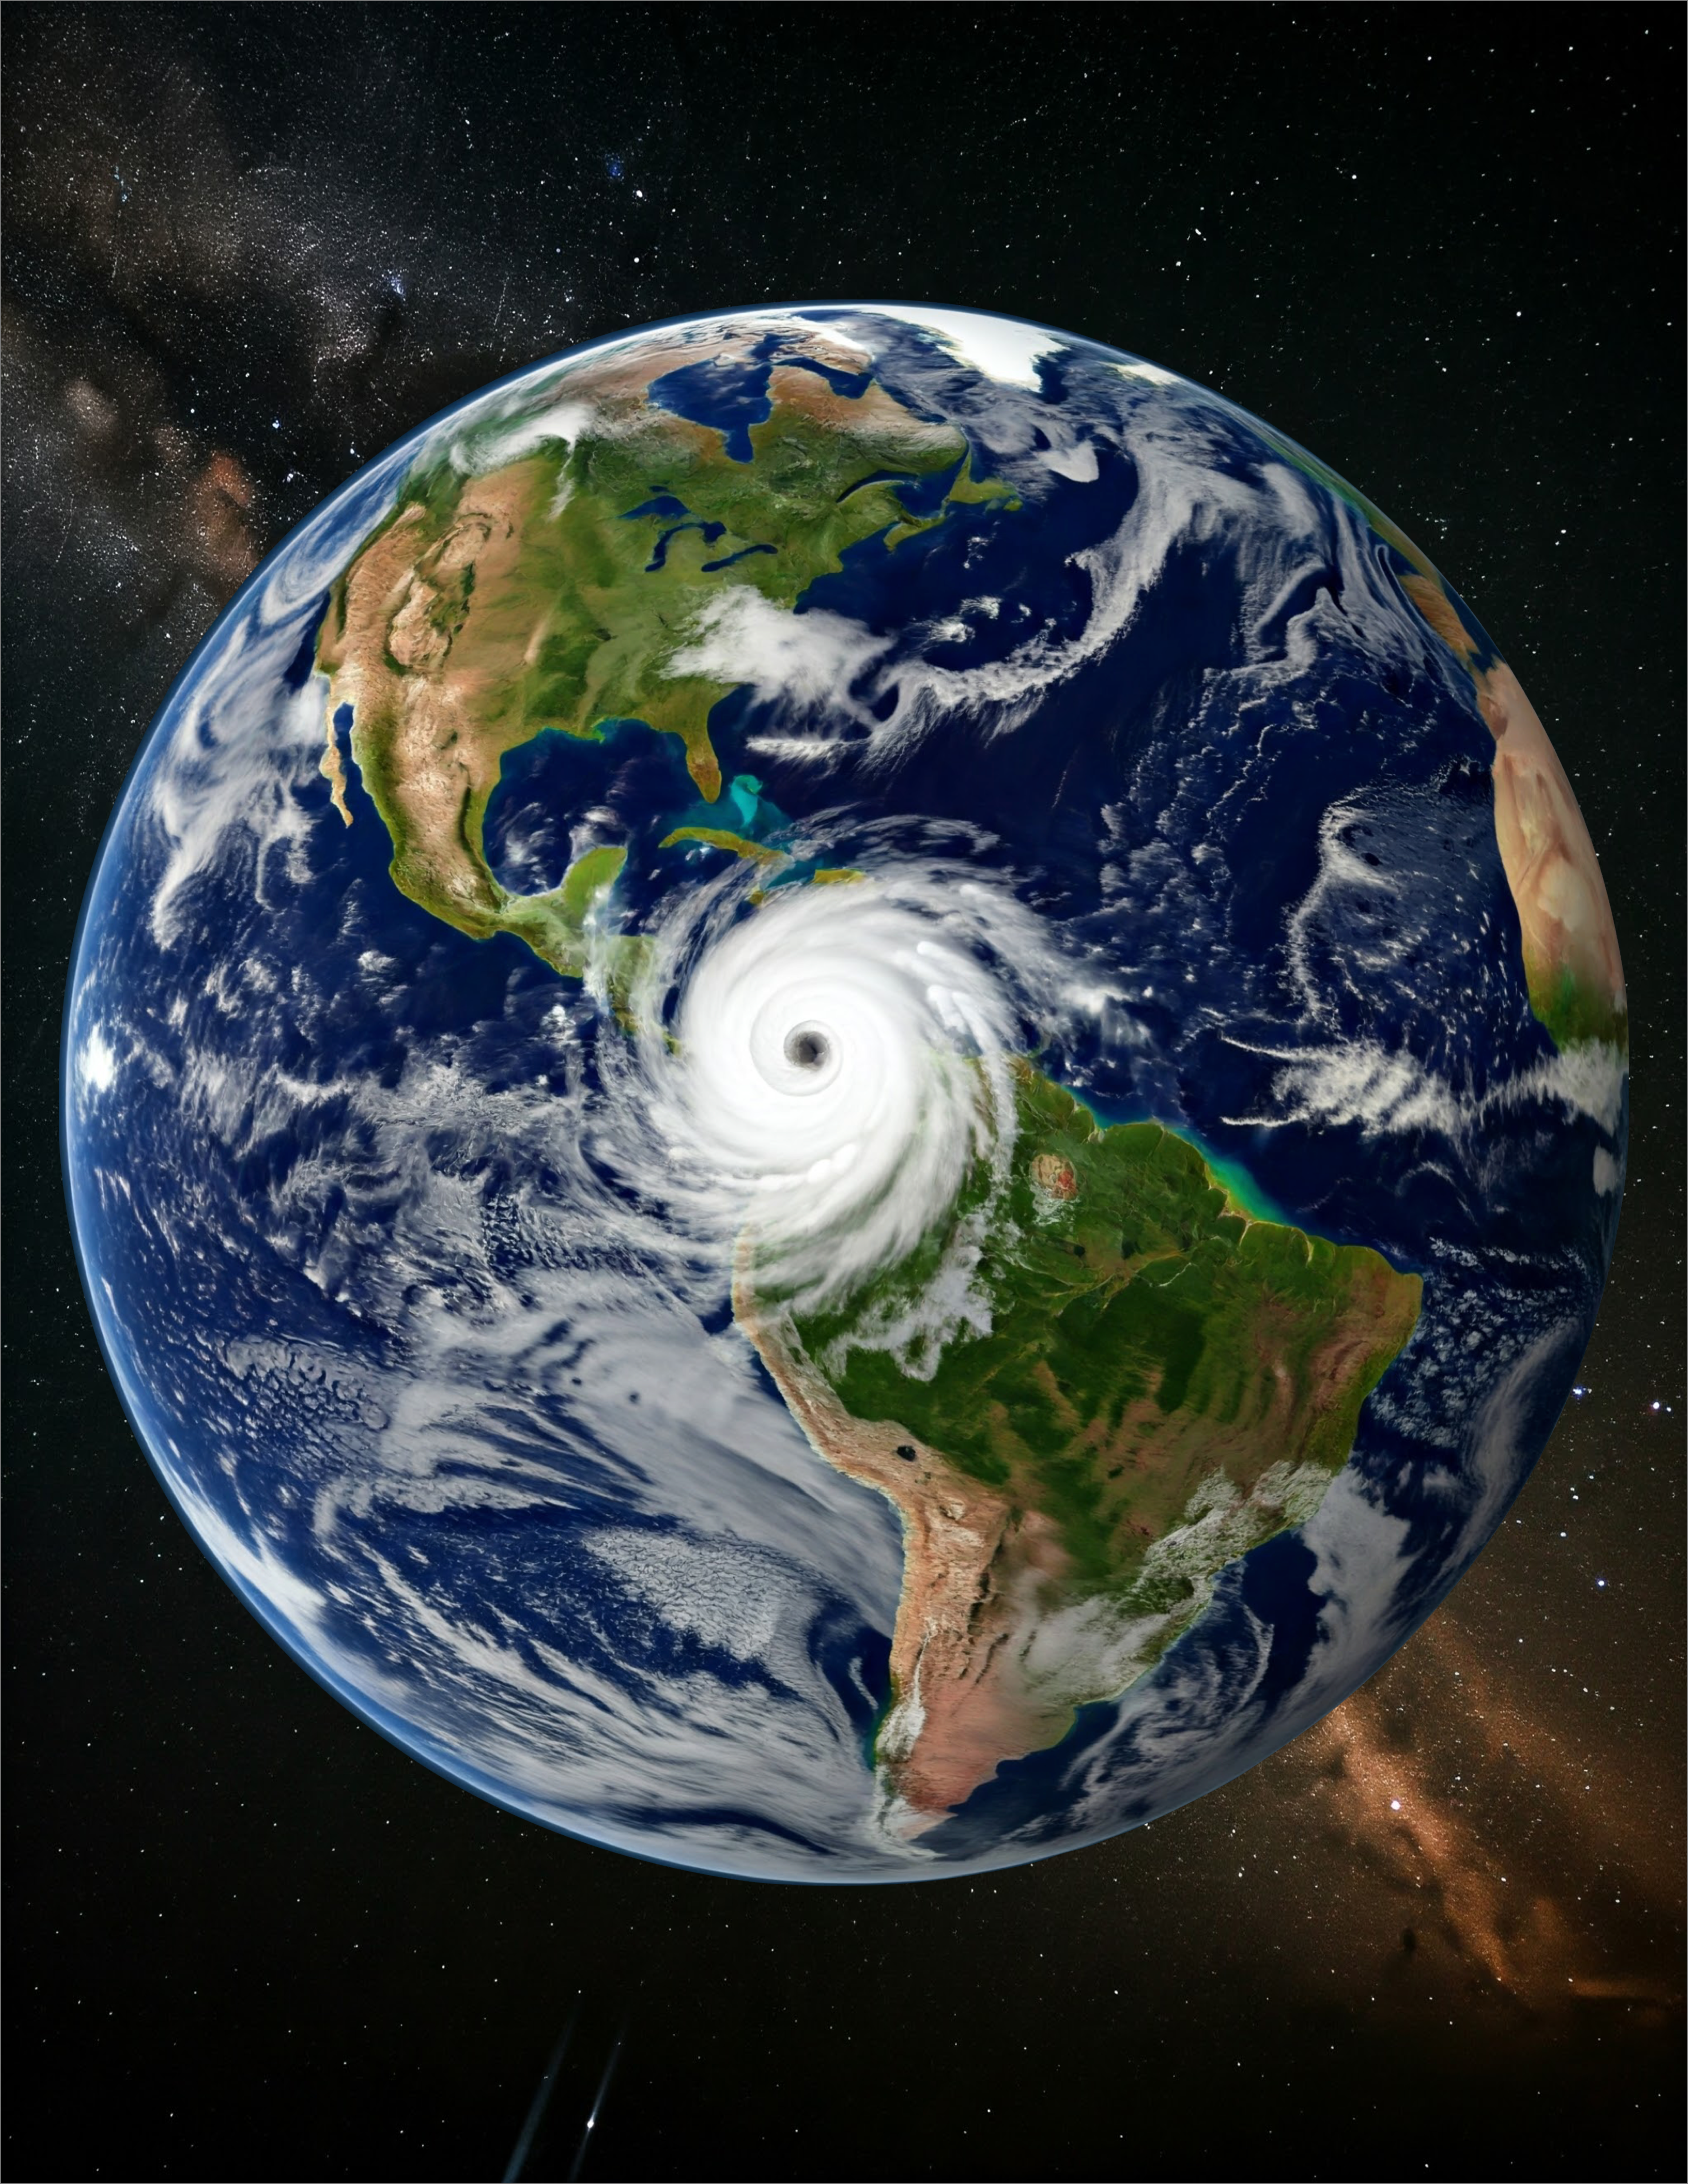
\includegraphics[width=\paperwidth, height=\paperheight]{images/Book-cover.pdf}};

%      \begin{scope}[
%        shift={(\pagewidth/2, -15cm)},
%        draw=white,
%        scale=1
%      ]
%        
%        % Define the vector field function
%        % Based on Van der Pol's equation with mu=0.08
%        \def\vectorfieldx(#1,#2){0.08 * (1 - (#2)^2) * (#1) - (#2)}
%        \def\vectorfieldy(#1,#2){(#1)}
%
%        % Draw the vector field
%        \foreach \x in {-10,-9.4,...,10}
%            \foreach \y in {-6,-5.4,...,6}
%            {
%                % Calculate the vector at (\x, \y)
%                \pgfmathsetmacro\vx{\vectorfieldx(\x,\y)}
%                \pgfmathsetmacro\vy{\vectorfieldy(\x,\y)}
%                
%                % Normalize the vector for consistent arrow lengths
%                \pgfmathsetmacro\norm{sqrt(\vx*\vx + \vy*\vy + 0.01)}
%                \pgfmathsetmacro\scaleChange{atan(\norm)/100/\norm}
%                \pgfmathsetmacro\vx{\vx*\scaleChange}
%                \pgfmathsetmacro\vy{\vy*\scaleChange}
%                            
%                % Draw the vector as an arrow
%                \draw[->] (\x,\y) -- ++(\vx,\vy);
%            }
%
%        
%      \end{scope}



		\fill[path fading=north,covershade] (0,2.2in) rectangle ([yshift=-1.01in, xshift=2pt]current page.north east);
		\fill[covershade] (0,-1in) rectangle ([yshift=-1.05in]current page.north east);
%		\fill[path fading=south, covershade] (0,-2in) rectangle ([xshift=1in,yshift=2in]current page.south east);
	\end{scope}		
\end{bigcover}




\newcommand{\titletext}[5]{
	\draw (#1, #2) node[right,opacity=0.55] {	
		\textpdfrender{
		    TextRenderingMode=Fill,
		    LineWidth=1pt,
		    FillColor=#4,
		  }{\fontsize{#5}{100}\fontfamily{phv}\selectfont  \bfseries #3}
	};
	\draw (#1, #2) node[right] {	
		\textpdfrender{
		    TextRenderingMode=Stroke,
		    LineWidth=1pt,
		    StrokeColor=#4,
		  }{\fontsize{#5}{100}\fontfamily{phv}\selectfont  \bfseries #3}
	};
}

\newcommand{\subtitletext}[5]{
	\draw (#1, #2) node[right,opacity=0.55] {	
		\textpdfrender{
		    TextRenderingMode=Fill,
		    LineWidth=1pt,
		    FillColor=#4,
		  }{\fontsize{#5}{100}\fontfamily{phv}\selectfont #3}
	};
	\draw (#1, #2) node[right] {	
		\textpdfrender{
		    TextRenderingMode=Stroke,
		    LineWidth=1pt,
		    StrokeColor=#4,
		  }{\fontsize{#5}{100}\fontfamily{phv}\selectfont #3}
	};
}




  \begin{scope}[yscale=-1, xscale=1, x=2.7pt, y=2.7pt,line join=miter,line cap=butt,line width=1.3pt, yshift=2.3cm, xshift=.7cm,
	  ]

	\coordinate (SUB) at (135, 4);

\begin{bookonly}
	\titletext{6}{-5}{Mathematical Modelling}{coverblue}{50}%{58}	
\end{bookonly}

\begin{displayonly}
	\titletext{6}{-5}{Mathematical Modelling}{coverblue}{45}%{50}	
\end{displayonly}


%    \begin{scope}[yscale=-9.7, xscale=9.7, yshift=-.96in]
%	  \fill[coverblue, opacity=.7] \LINEARALGEBRAoutline;
%	  \draw[coverblue, line width=1.3pt] \LINEARALGEBRAoutline;
%    \end{scope}
  \end{scope}
%


  

	\path[white] (SUB) node[anchor=north west] {\Large \bfseries \sffamily \coversubtitle};



\newcommand{\authornames}{\huge \sffamily \bfseries \begin{tabular}{r}Bernardo Galv\~ao-Sousa\end{tabular}}
	\newcommand{\ypadd}{.5em}
	\newcommand{\xpadd}{1em}


\begin{bookonly}
	\draw (0, 15) node[right, xshift=10em] (AUTHOR) {\phantom{\authornames}};	
\end{bookonly}
\begin{bigcover}
	\draw (0, -25) node[right, xshift=10em] (AUTHOR) {\phantom{\authornames}};		
\end{bigcover}

\begin{displayonly}
	\draw (0, -8.5) node[right, xshift=10em] (AUTHOR) {\phantom{\authornames}};	
\end{displayonly}

\begin{slidesonly}

	\path let \p1 = (AUTHOR.north) in coordinate (Ab1) at (0,\y1+\ypadd);
	\path let \p1 = (AUTHOR.north east) in coordinate (Ab2) at (\x1+\xpadd,\y1+\ypadd);
	\path let \p1 = (AUTHOR.south east) in coordinate (Ab3) at (\x1+\xpadd,\y1-\ypadd);
	\path let \p1 = (AUTHOR.south) in coordinate (Ab4) at (0,\y1-\ypadd);

	\path[fill=covershade, path fading=west, opacity=.8] (Ab1) -- (Ab2) -- (Ab3) -- (Ab4);
	\draw[covershade!80!black, line width=1.3pt] (Ab1) -- (Ab2) -- (Ab3) -- (Ab4);
	
	\draw (0, -8.5) node[right, xshift=10em, white!75!black] (AUTHOR) {\authornames};	
\end{slidesonly}

\begin{bookonly}
	\draw (0, 15) node[right, xshift=10em, white!75!black] (AUTHOR) {\authornames};
\end{bookonly}
\begin{bigcover}
	\path let \p1 = (AUTHOR.north) in coordinate (Ab1) at (0,\y1+\ypadd-470);
	\path let \p1 = (AUTHOR.north east) in coordinate (Ab2) at (\x1+\xpadd,\y1+\ypadd-470);
	\path let \p1 = (AUTHOR.south east) in coordinate (Ab3) at (\x1+\xpadd,\y1-\ypadd-470);
	\path let \p1 = (AUTHOR.south) in coordinate (Ab4) at (0,\y1-\ypadd-470);

	\path[fill=covershade, path fading=west, opacity=.8] (Ab1) -- (Ab2) -- (Ab3) -- (Ab4);
	\draw[covershade!80!black, line width=1.3pt] (Ab1) -- (Ab2) -- (Ab3) -- (Ab4);

	\draw (0, -25) node[right, xshift=10em, white!75!black] (AUTHOR) {\authornames};
\end{bigcover}

\end{tikzpicture}


\newpage

\begin{bookonly}
	\clearpage
	\hbox{}
	\newpage
	\input{modules/preface.tex}
	\section*{Contributors}
	\input{common/contributors.tex}
%	\section*{Dedication}
%	\begin{center}
%		This book is dedicated to
%		\href{https://www.gazettetimes.com/news/local/obituaries/dr-robert-main-burton/article_9c087f07-c005-515a-bb3f-2c9c6a6b7332.html}{\color{blue}Dr.~Bob Burton}---friend and mentor.
%
%		\emph{\large ``Sometimes you have to walk the mystical path with practical feet.''}
%	\end{center}
	\newpage
	\mbox{}
	{
		\pagestyle{empty}
		\setcounter{tocdepth}{1}
		\tableofcontents
		\thispagestyle{empty}
	}
	\newpage
	\mbox{}
	\newpage
\end{bookonly}

\setcounter{page}{1}
\pagestyle{siefken}


\addcontentsline{toc}{chapter}{Lessons}

\begin{module}\label{module1}
	\Title{Modeling}

	In this module you will learn
	\begin{itemize}
		\item ??
	\end{itemize}

	\input{modules/module1.tex}
	%\input{modules/module1-exercises.tex}
\end{module}





\begin{slide}

\question 

\begin{parts}
	\item What is modelling?
\end{parts}



\begin{solution}
	\begin{itemize}
		\item A precise description of a system
		\item A formal summary of knowledge
		\item A tool that enables prediction
		\item An abstraction suitable for a particular purpose or question
		\item Modelling is a scientific method with ``hypothesis'' in a mathematical form	
	\end{itemize}	
\end{solution}
	
\end{slide}




\begin{slide}
\begin{parts}
\setcounter{partsitem}{1}
	\item Modelling Procedure -- DABAR \footnote{based on the \href{SIAM $M^2 (GS)^2$ Textbook}{https://m3challenge.siam.org/wp-content/uploads/siam-guidebook-final-press.pdf}.}
	
	\begin{enumerate}
		\item[\it Step 1.] \textbf{\large D}efine the problem 
			\begin{solution}\hfill (ask a question)\end{solution}

		\item[\it Step 2.] make \textbf{\large A}ssumptions 
			\begin{solution}\hfill (select a modelling approach)\end{solution}

		\item[\it Step 3.] \textbf{\large B}uild a model
			\begin{solution} \hfill (formulate the model)\end{solution}

		\item[\it Step 4.] \textbf{\large A}ssess the model 
			\begin{solution} \hfill (solve the model) \end{solution}

		\item[\it Step 5.] \textbf{\large R}eport results
			\begin{solution} \hfill (answer the question) \end{solution}
	\end{enumerate}	
\end{parts}

	
\end{slide}




\begin{slide}

\begin{parts}
\setcounter{partsitem}{2}

	\item Course topics:

\begin{itemize}
	\item Optimization models
	\item Dynamics models
	\item Probability models
\end{itemize}
	
\end{parts}

\end{slide}




%%%%%%%%%%%%%%%%%%%%%%%%%%%%%%%%%%%%%%%%%%%%%%%%%%%%%
%
%
%  	OPTIMIZATION MODELS
%
%
%%%%%%%%%%%%%%%%%%%%%%%%%%%%%%%%%%%%%%%%%%%%%%%%%%%%%




\begin{slide}

\begin{slidesonly}
	\vspace{3cm}
\end{slidesonly}

\begin{center}
\Huge 
\textcolor{LimeGreen}{Optimization Models}
\end{center}

	
\end{slide}




\begin{slide}

\question

\begin{problem}[Optimization Problem\footnote{Adapted from ``Mathematical Modelling'' by Meerschaert.}]
A pig weighting 90 kg gains 3 kg per day and cost 45 cents a day to keep. The market price for pigs is 65 cents/kg, but is falling at 1 cent per day. When should the pig be sold?	
\end{problem}

Introduce variables:
\begin{itemize}
	\item $t=$ time at which the pig is sold (in days)
	\item $w=$ weight of the pig (in kg)
	\item $m=$ market price of a pig (in \$/kg)
	\item $C=$ cost of keeping the pig (in \$)
	\item $R=$ revenue from selling the pig (in \$)
	\item $P=$ profit from the sale of the pig (in \$)
\end{itemize}
	

\begin{parts}
	\item Which of these variables depend on $t$? Based on the statement, what do we know about their values?
	\item What is our goal?
	\item Solve the problem.
	\item Answer the question: when should the pig be sold and what is the profit?
\end{parts}

\end{slide}

\begin{slide}

\SavedDefinitionRender{Sensitivity}

\textbf{Example:} If the time to sell or the profit depends strongly on a parameter, then the model is not very useful.
If the model said to sell at $t=1$ if the daily maintenance cost changed to 46 cents, then the recommendation would be very suspect!

\begin{parts}
\setcounter{partsitem}{4}

	\item Let $(t^\star,P^\star)$ be the optimal values found before. 
	
	What is the sensitivity of $P$ over the parameter $c_d=$ the daily maintenance cost of keeping a pig?
	
	\item Is $S(P^\star,c_d)$ positive/negative? What does that mean? Does that make sense?
	
	\item What is the sensitivity of $P$ over the parameter $m_0=$ the initial market price of a pig (in \$/kg)?

	\item Is $S(P^\star,m_0)$ positive/negative? What does that mean? Does that make sense?

\end{parts}

\end{slide}


\begin{solution}
\begin{slide}
\textbf{Solutions:}
\begin{parts}
	\item 
	\begin{itemize}
 		\item $w(t) = 90 + 3t$
 		\item $m(t) = 0.65-0.01t$
 		\item $C(t) = 0.45t$
 		\item $R(t) = p(t) \cdot w(t)$
 		\item $P(t) = R(t) - C(t)$
 	\end{itemize}
 	\item The goal is to maximize $P(t)$ over $t\geq 0$.
 	\item 	$P(t) = (90+3t)(0.65-0.01t) - 0.45t$ \\
			$\dfrac{dP}{dt} = 3(0.65-0.01t)-0.01(90+3t) - 0.45 = 0$\\
 			$t^\star = 10$ \\	
 			$P^\star(10) = 61.50$
 	\item The pig should be sold on day 10, which will give a profit of \$61.50.

%	\item We have $P = (90+3t)(0.65-0.01t) - c_dt$ and $t^\star = \frac{35}{2} - \frac{50}{3} c_d$.
%
%		We get $P^\star = \frac{25}{3} c_d^2 - \frac{35}{2} c_d + \frac{1083}{16}$ so that
%		\begin{align*}
%		S(P^\star,c_d) 
%			& = \frac{\partial P^\star}{\partial c_d} \frac{c_d}{P^\star} \big|_{c_d=0.45} \\
%			& = \frac{\frac{50}{3} c_d^2 - \frac{35}{2}c_d}{\frac{25}{3} c_d^2 - \frac{35}{2} c_d + \frac{1083}{16}}\big|_{c_d=0.45}
%			= -0.0731707
%		\end{align*}
	\item We have $P = (90+3t)(0.65-0.01t) - c_dt$ so that
		\begin{align*}
		S(P^\star,c_d) 
			& = \frac{\partial P^\star}{\partial c_d} \frac{c_d}{P^\star} \big|_{c_d=0.45} \\
			& = - t^\star \frac{c_d}{P^\star} \big|_{c_d=0.45}
			= -0.0731707
		\end{align*}
		This model is insensitive with respect to the maintenance cost! =)
	\item It is negative, which means that increasing the daily maintenance cost will decrease the profit, which makes sense.
	
	\item We get $S(P^\star,m_0) = 1.26829$, so
%
%		We have $P = (90+3t)(m_0-0.01t) - 0.45t$ and $t^\star = 50m_0-\frac{45}{2}$.
%
%		We get $P^\star = 75 m_0^2 + 22.5 m_0 + 15.1875$ so that
%		\begin{align*}
%		S(P^\star,m_0) 
%			& = \frac{\partial P^\star}{m_0} \frac{m_0}{P^\star} \big|_{m_0=0.65} \\
%			& = \frac{150m_0^2 + 22.5m_0}{75 m_0^2 + 22.5 m_0 + 15.1875}\big|_{m_0=0.65}
%			= 1.26829
%		\end{align*}
		this model is moderately sensitive to the initial price for a pig. =/
		
	\item The sensitivity is positive since increasing the initial price of a pig increases the profit also.
	
\end{parts}


	
\end{slide}

\end{solution}



\begin{slide}

\begin{definition}[Robustness]
How do the results depend on the assumptions?\\

We assumed:
\begin{itemize}
	\item a linear increase in weight of the pig
	\item a linear decrease in the price of the pig	  \\
\end{itemize}
%\hfill\\

What happens if these were nonlinear? The prediction of prices is notoriously uncertain. \\

Prices are often modelled as stochastic processes (like Brownian motion). This would necessitate a different modelling approach.  \\

In particular, we might then want to maximize the expected (average) profit. But if the variance is very large, then the farmer might prefer a lower expected profit if that means lowering the risk (variance). 
The farmer might consider maximizing the expected profit with a constraint on the variance of the profit.
\end{definition}

\end{slide}








\begin{slide}

\question 

\begin{problem}%[Unconstrained Optimization]
	A manufacturer of lawn furniture makes two types of chairs, one with a wood frame and the other with an aluminum frame. The wood frame chair costs \$18 per unit to manufacture and aluminum frame chair costs \$10 per unit to manufacture. The company operates in a market where the number of units that can be sold depends on price. It is estimated that in order to sell $x$ units per day of the wood chair and $y$ units per day of the aluminum chair, the selling price cannot exceed $10 + 31x^{-0.5} + 1.3y^{-0.2}$ dollars per unit for the wood chair and $5 + 15y^{-0.4} + 0.8x^{-0.08}$ dollars per unit for the aluminum chair.
\end{problem}


Let us first investigate the selling price model for \textbf{one type of} chair. %: $P = c_0 + c_1 x^{-a} + c_2 y^{-b}$.

\begin{parts}
	\item As more chairs of both types are sold in the market: $x \to \infty$, what do you expect will happen to their selling price?
	
%	$$ P \to {\rm Cost}$$
	
	\item As chairs become scarce: $x \to 0^+$, what happens to the price?
	
%	$$P \to \infty$$
	
	\item What family of functions satisfies both these conditions?
	
%	$$P = c_0 + c_1 x^{-b}$$
	
\end{parts}
 

%\SavedDefinitionRender{LagrangeMultipliers}
	
\end{slide}


\begin{slide}

\begin{center}
\includegraphics[width=0.6\textwidth]{images/fitprice.png}

Historical prices and fitting surface $p=f(x,y)$.
\end{center}

\end{slide}



\begin{slide}

\question

\begin{problem}%[Unconstrained Optimization]
	A manufacturer of lawn furniture makes two types of chairs, one with a wood frame and the other with an aluminum frame. The wood frame chair costs \$18 per unit to manufacture and aluminum frame chair costs \$10 per unit to manufacture. The company operates in a market where the number of units that can be sold depends on price. It is estimated that in order to sell $x$ units per day of the wood chair and $y$ units per day of the aluminum chair, the selling price cannot exceed $10 + 31x^{-0.5} + 1.3y^{-0.2}$ dollars per unit for the wood chair and $5 + 15y^{-0.4} + 0.8x^{-0.08}$ dollars per unit for the aluminum chair.
\end{problem}


\begin{parts}
	\item We want to maximize the manufacturer's profit. What is the function to maximize?
	\item This is a two-dimensional function, so we need to solve the system
	\begin{align*}
		\frac{\partial f}{\partial x} & = 0 \\[5pt]
		\frac{\partial f}{\partial y} & = 0		
	\end{align*}

	Write down this system.
	\item How can we find the solution?
\end{parts}
	
\end{slide}



\begin{slide}

\SavedDefinitionRender{Newton1}
\begin{minipage}{0.6\textwidth}
	
\begin{parts}
\setcounter{partsitem}{3}
	\item From the description above, sketch the point $x_1$ on the graph on the right when using Newton's method.
	
	\item What is the formula for $x_1$?
	
\begin{slidesonly}
	\bigskip
\end{slidesonly}
	
	\item Leveraging python.
	\begin{enumerate}
%		\item Go to \url{https://utoronto.syzygy.ca/jupyter}
%		\item Download the file \href{https://raw.githubusercontent.com/bigfatbernie/IBLMathModeling/main/python/chairs_newton.ipynb}{\tt chairs\_newton.ipynb} and import it into the Jupyter Notebook
		\item Clone the file \href{https://utoronto.syzygy.ca/jupyter/user-redirect/git-pull?repo=https://github.com/bigfatbernie/IBLMathModeling&subPath=python/chairs_newton.ipynb}{\tt chairs\_newton.ipynb} into your Jupyter Notebook
		\item In the file, introduce the partial derivative functions and an initial guess.
		\item Run the script
	\end{enumerate}
\end{parts}
\end{minipage}
\hfill
	\begin{minipage}{0.35\textwidth}
		\begin{tikzpicture}%[scale=0.65]
		  \draw[-latex] (0,-1.5) -- (0,2.5);
		    \draw[-latex] (-0.25,0) -- (6,0);
		%    \draw[ultra thick, blue, variable=\x, samples=100,domain=0:8] plot ({\x},{(-1.5*sin(180*(\x-4.5)/pi)*(\x-4.5+0.1(\x-4.5)^3-3*(\x-4.5))/4});
		    \draw[ultra thick, blue, variable=\x, samples=100,domain=-0.25:6] plot ({\x},{(-1.5*sin(180*(\x-4.5)/pi)*(\x-4.5)+0.1*(\x-4.5)^3-3*(\x-4.5)-0.2)/5});
		  \draw[dashed, thick] (2,{(-1.5*sin(180*(2-4.5)/pi)*(2-4.5)+0.1*(2-4.5)^3-3*(2-4.5)-0.2)/5}) -- (2,0) node[below] {$x_0$};
		  \draw[ultra thick, green!50!black, fill=green!75!black] (2,{(-1.5*sin(180*(2-4.5)/pi)*(2-4.5)+0.1*(2-4.5)^3-3*(2-4.5)-0.2)/5}) circle (0.1);
		\end{tikzpicture}
	\end{minipage}

\end{slide}


\begin{slide}

\includegraphics[width=.75\textwidth]{images/chairs-profit.png}
	
\end{slide}

\begin{slide}

\begin{parts}
\setcounter{partsitem}{5}
	\item Leveraging python's minimization tools.
	\begin{enumerate}
%		\item Go to \url{https://utoronto.syzygy.ca/jupyter}
%		\item Download the file \href{https://raw.githubusercontent.com/bigfatbernie/IBLMathModeling/main/python/chairs_fmin.ipynb}{\tt chairs_fmin.ipynb} and import it into Jupyter Notebook
		\item Clone the file \href{https://utoronto.syzygy.ca/jupyter/user-redirect/git-pull?repo=https://github.com/bigfatbernie/IBLMathModeling&subPath=python/chairs_fmin.ipynb}{\tt chairs\_fmin.ipynb} into your Jupyter Notebook
		\item In the file, introduce the profit function and an initial guess.
		\item Run the script
	\end{enumerate}
\end{parts}
\end{slide}


\begin{slide}

\question

\begin{problem}%[Unconstrained Optimization]
	A manufacturer of lawn furniture makes two types of chairs, one with a wood frame and the other with an aluminum frame. The wood frame chair costs \$18 per unit to manufacture and aluminum frame chair costs \$10 per unit to manufacture. The company operates in a market where the number of units that can be sold depends on price. It is estimated that in order to sell $x$ units per day of the wood chair and $y$ units per day of the aluminum chair, the selling price cannot exceed $10 + 31x^{-0.5} + 1.3y^{-0.2}$ dollars per unit for the wood chair and $5 + 15y^{-0.4} + 0.8x^{-0.08}$ dollars per unit for the aluminum chair.
\end{problem}


\textbf{Sensitivity}. To compute $p^\star$, you can use \href{https://utoronto.syzygy.ca/jupyter/user-redirect/git-pull?repo=https://github.com/bigfatbernie/IBLMathModeling&subPath=python/chairs_sensitivity.ipynb}{\tt chairs_sensitivity.ipynb}.

\begin{parts}
	\item How sensitive is the profit to the parameter $c = 10$ (the production cost of the aluminum chair)
		\[ S(p^\star, c) %= \frac{\partial S}{\partial c} (p^\star,c) \cdot \frac{c}{p^\star(c)} 
			\approx \frac{p^\star(c+h) - p^\star(c)}{h} \cdot \frac{c}{p^\star(c)}?
		\]

	\item How sensitive is the profit to the parameter $b = 0.4$ (the exponent of $y$ in the selling price of the aluminum chair)
		\[ S(p^\star, b) \approx \frac{p^\star(b+h) - p^\star(b)}{h} \cdot \frac{b}{p^\star(b)}?
		\]
\end{parts}

% We already calculated all the terms in these expressions for S except the $p^\star(b+h)$. Those are the only ones we need to calculate.

\begin{solution}
\hspace{-3em}Note that we are using numerical derivatives, since calculating the partial derivatives analytically is usually impossible.	
\end{solution}



\end{slide}






\begin{slide}

\question

\textbf{Constrained Optimization.} 
How do we solve optimization problems with constraints?

\SavedDefinitionRender{LagrangeMultipliers}


\begin{definition}[Notes:]
\begin{enumerate}
	\item This is a necessary, but not sufficient condition.
	\item To solve the optimization problem, find candidates $x$ that satisfy it, and then pick the best one.
	\begin{itemize}
		\item Points for which $\nabla g_1(x), \ldots, \nabla g_k(x)$ are linearly dependent should also be candidates.
	\end{itemize}
	\item \eqref{LM} $\Leftrightarrow \nabla f(x^\star) \in {\rm span}\Big\{\nabla g_1(x), \ldots, \nabla g_k(x)\Big\}$.
	\item The ``optimal'' values for $\lambda_1, \ldots, \lambda_k$ give important insights on the problem, as we will see -- don't ignore them!
\end{enumerate}
\end{definition}

\end{slide}





\begin{slide}
	
\begin{problem}[Example]
Consider the problem:
\begin{itemize}
	\item Maximize $x+y$ \quad such that $x^2+y^2 = 1$.
\end{itemize}
\end{problem}

\begin{center}
	\includegraphics[width=.4\textwidth]{images/LagrangeMultipliers-ex.png}
\end{center}

\begin{parts}
	\item Use Lagrange Multipliers to find the maximum (and the minimum).

	\item If the constraint was $x^2+y^2=c$, then what is:
	\begin{enumerate}
		\item the maximizer point $(x^\star,y^\star)$?
		\item the Lagrange multiplier $\lambda^\star$?
		\item the maximum $f(x^\star,y^\star)$?
	\end{enumerate}
	
	\item Compare $\lambda^\star$ with $\dfrac{\partial f(x^\star,y^\star)}{\partial c}$.
	
	\item Based on this relation, give an interpretation for the Lagrange Multiplier.
	
\end{parts}

\end{slide}


\begin{solution}
\begin{slide}

\begin{parts}
	\item 
	\begin{align*}
		\nabla f & = \mat{1\\1}  
			\quad \text{ and } \quad \nabla g = \mat{2x\\2y} \\
		\\
		\mat{1\\1} & = \lambda \mat{2x \\ 2y} \quad \Leftrightarrow \quad 
			\begin{cases}
				1 & = 2\lambda x \\
				1 & = 2\lambda y \\
				1 & = x^2 + y^2	
			\end{cases}
			\\
		1 & = \frac{1}{2 \lambda^2} \quad \Leftrightarrow\quad 
			\lambda = \pm\frac{1}{\sqrt{2}}\\
		x & = y = \pm \frac{1}{\sqrt{2}}
	\end{align*}
	
	\item $x^\star=y^\star= \frac{\sqrt{c}}{\sqrt{2}}$ \quad and \quad $\lambda^\star = \frac{1}{\sqrt{2c}}$
		 
		 $\max = x^\star+y^\star=\sqrt{2c}$
		
	\item $\dfrac{\partial f(x^\star,y^\star)}{\partial c}
			= \dfrac{\sqrt{2}}{2\sqrt{c}} = \lambda^\star$

	\item This means that if the constraint increased from $1$ to $1 + \Delta = 1.1$, 	then we would expect the maximum to increase by approximately $\Delta \lambda^\star = \frac{\Delta}{\sqrt{2}} \approx 0.07$.
		
		Indeed, $\Delta f = \sqrt{2.2}-\sqrt{2} \approx 0.069$.

\end{parts}
	
\end{slide}	
\end{solution}


%\begin{solution}
%\begin{slide}
%
%We obtain the following equations:
%\begin{align*}
%	\nabla f & = \mat{1\\1} \\	
%	\nabla g & = \mat{2x\\2y} \\
%	\\
%	\mat{1\\1} & = \lambda \mat{2x \\ 2y} \\
%	\\
%	1 & = 2\lambda x \\
%	1 & = 2\lambda y \\
%	1 & = x^2 + y^2 \\
%	\\
%	1 & = \frac{1}{2 \lambda^2} \\
%	\lambda & = \pm\frac{1}{\sqrt{2}}\\
%	x & = y = \pm \frac{1}{\sqrt{2}}
%\end{align*}
%		
%\end{slide}
%\end{solution}









\begin{slide}

\question

\textbf{Define the problem.}

\begin{problem}
The production side of the electrical power grid\footnote{This example is based on \href{https://sces.phys.utk.edu/~moreo/mm08/method_HLi.pdf}{Huijuan Li in `Lagrange Multipliers and their Applications'}.} consists of hundreds or thousands of power plants that vary in fuel sources (coal, nuclear, hydroelectric, solar, wind, stored energy in the batteries of electric vehicles, etc.) and characteristics (age, efficiency, automated, etc.). 

How can the power consumption load be allocated to these plants to minimize cost?
\end{problem}


\textbf{Make Assumptions.}

\begin{itemize}
	\item Each power plant is summarized by a cost curve which tells how much a given load costs. Generally, the cost per unit time per unit load of operating a power plant is a concave function of load as in the figure below: small and large loads are expensive.
	\item For simplicity, we will approximate these quadratics by a linear function with one parameter: the cost per unit time per unit load is $c(x) =ax+1$, so the cost rate function has the form $f(x)=(ax+1)x = ax^2+x$.
	
	\includegraphics[width=.4\textwidth]{images/concavecost.png} 
	
	\item $N=$ number of power plants
	\item $x_i=$ load assigned to power plant $i$ (in MW)
	\item $X=$ total load (in MW)({In Toronto the average total load is 2500 MW.}).
	\item $C=$ cost rate of power generation (in \$/h)
	\item $f_i(x_i)=$ cost rate function for power plant $i$ (in \$/h)
	

\end{itemize}

	
\end{slide}


\begin{slide}

\textbf{Build a model.}

\begin{parts}
	\item Find an equation relating $X$ and $x_i$.
	\item Find a formula for $C$.
	\item Formulate the problem we want to solve.
	

\begin{slidesonly}
	\bigskip
\end{slidesonly}

\hspace{-2em}
\textbf{Assess the model.}

\hspace{-2em}
	We are going to assume the following:
	\begin{itemize}
		\item Three power plants identified with the parameters:
		\begin{itemize}
			\item $a_1 = 0.0625 $
			\item $a_2 = 0.0125 $
			\item $a_3 = 0.0250 $
		\end{itemize}
		\item The total load is 925 MW
	\end{itemize}


	\item Solve the problem.

\begin{slidesonly}
	\vspace{5cm}
\end{slidesonly}

\hspace{-2em}
\textbf{Report the results.}

	\item What is the interpretation of $\lambda^\star$ the ``optimal'' Lagrange multiplier?
	\item What is the sensitivity of the cost with respect to the parameters $a_i$ and $X$? What does that mean about the model?
		
\end{parts}
	
\end{slide}


\begin{solution}
\begin{slide}

\begin{parts}
\setcounter{partsitem}{2}
	\item 	
		\begin{tabular}[t]{ll}
			Objective: 	& $\displaystyle \min \quad \sum_{i=1}^3 a_i x_i^2 + x_i$ \\
			Constraint: & $\displaystyle \sum_{i=1}^3 x_i = X$
		\end{tabular}

	\item Define:
		\begin{align*}
			C(\vec{x}) & = \sum_{i=1}^3 a_i x_i^2 + x_i \\
			g(\vec{x}) & = \sum_{i=1}^3 x_i = X
		\end{align*}
		
		So we have
		\[
			\nabla C (\vec{x}) 
				= \mat{2a_1 x_1 + 1\\2a_2 x_2 + 1\\2a_3 x_3 + 1} 
				= \lambda	\nabla g (\vec{x}) 
				= \lambda \mat{1\\1\\1}
		\]
		
		Which can be written as
		\[ \matc{2a_1 & 0 & 0 & -1\\0 & 2a_2 & 0 & -1\\0 & 0 & 2a_3 & -1 \\ 1 & 1 & 1 & 0} \mat{x_1\\x_2\\x_3\\\lambda} = \mat{-1\\-1\\-1\\ X}
		\]
		
		And we get the unique solution:
		\begin{itemize}
			\item $x_1 = 112$ MW
			\item $x_2 = 560$ MW
			\item $x_3 = 280$ MW
			\item $\lambda = \$15$ /h/MW (shadow cost)
		\end{itemize}
		
		We used: \href{https://utoronto.syzygy.ca/jupyter/user-redirect/git-pull?repo=https://github.com/bigfatbernie/IBLMathModeling&subPath=python/power-plants.ipynb}{\tt power-plants.ipynb}
		
		\item If we reduce the total load ($X$) by 1 MW, it would approximately reduce the total cost of operating the three power plants by \$15/h.
		
		So the operator of the power plants should be willing to pay consumers who pump electricity back to the grid up to \$15/h for each megawatt.

		\item 	\begin{itemize}
			\item $S(C,X) \approx 1.875$
			\item $S(C,a_1) \approx 0.000015$
			\item $S(C,a_2) \approx 0.00017$
			\item $S(C,a_3) \approx 0.00007$
		\end{itemize}


	
\end{parts}
	
\end{slide}
	
\end{solution}


\begin{slide}

\question

\textbf{Robustness.} 

\begin{parts}
	\item The parameter $X$ varies significantly (regularly by over 50\% in a day), so understanding it is very important.

\begin{center}
	\includegraphics[width=0.4\textwidth]{images/energydemand.png}
\end{center}
	

It is crucial to understand how the optimal cost and loads change with $X$.


	\item Is the quadratic model for $f_i$ good? You can try different functions.
	\item Should there be other constraints on $x_i$? We only imposed $x_i>0$, but we probably should impose upper bounds too.
	\item What about transportation costs? There can be losses of up to 20\% on high-tension transmission lines.
	\item We have a static model, where the power plants operate always at the same load. We might want to consider a dynamic optimization model.
\end{parts}



\end{slide}







\begin{slide}
\question

\begin{problem}[Linear Programming\footnote{based on a problem from Meerschaert's `Mathematical Modeling'.}]
	A family farm has 1250 hectares\footnote{1 hectare $=1$ ha $=$ 10\,000 m$^2$.}  of land for planting. Possible crops that they could plant are corn, wheat, and oats. There are 400 hectare-m (a volume) of water available for irrigation and 600 hours of labour per week available. The requirements and expected yields are shown below.
	
	
	\begin{center}
	\small
	\begin{tabular}{l|c|c|c}
	%\hline
	& corn & wheat & oats \\ \hline
	irrigation (ha-m / ha) & 1.0 & 0.3 & 0.5 \\ \hline
	labour (person-h / week / ha) & 1.6 & 0.4 & 0.6 \\ \hline
	yield (\$/ha) & 1400 & 420 & 700 \\ %\hline
	\end{tabular}
	\end{center}
	
	We want to maximize the total yield.
\end{problem}

Introduce the following variables:
\begin{itemize}
	\item $x_i= $ hectares planted of $i=1$ corn, $i=2$ wheat, $i=3$ oats
	\item $w=$ the total irrigation used in ha-m
	\item $\ell=$ the total labour used in person-h / week
	\item $a=$ the total area planted in hectares
	\item $y=$ the total yield in \$
\end{itemize}

\begin{parts}
	\item Find expressions for $w, \ell, a, y$
	\item What are the constraints on the variables defined?	
	\item Formulate the optimization problem we want to solve in standard linear programming form:
	\begin{center}
		\begin{tabular}{lc}
		Objective: 		& max \ $\vec{c}^T \vec{x}$ \\
		\multirow{2}{*}{Constraints:} 	& $A \vec{x} \leq \vec{b}$ \\
						& $\vec{x} \geq \vec{0}$
		\end{tabular}
	\end{center}
	\item Use \href{https://utoronto.syzygy.ca/jupyter/user-redirect/git-pull?repo=https://github.com/bigfatbernie/IBLMathModeling&subPath=python/farm-linearprog.ipynb}{\tt farm-linearprog.ipynb} to find the solution.

\end{parts}

\end{slide}


\begin{solution}
\begin{slide}
\begin{parts}
	\item
		\begin{itemize}
			\item $w = 1x_1 + 0.3x_2 + 0.5 x_3$
			\item $\ell = 1.6 x_1 + 0.4 x_2 + 0.6 x_3$
			\item $\displaystyle a = \sum_{i=1}^3 x_i$
			\item $y = 1400 x_1 + 420 x_2 + 700 x_3$
		\end{itemize}
		
	\item 
		\begin{itemize}
			\item $x_i \geq 0$
			\item $w \leq 400$
			\item $\ell \leq 600$
			\item $a \leq 1250$
		\end{itemize}
	\item 	\begin{tabular}[t]{lc}
				Objective: 						& max \ $\mat{1400 & 420 & 750} \vec{x}$ \\
				\multirow{2}{*}{Constraints:} 	& $\mat{1 & 0.3 & 0.5\\1.6 & 0.4 & 0.6\\1 & 1 & 1} \vec{x} \leq \mat{400\\600\\1250}$ \\
							& $\vec{x} \geq \vec{0}$
			\end{tabular}
\end{parts}
\end{slide}
\end{solution}

\begin{slide}

We ran the same model with the Wheat Yield ranging from \$400/ha to \$440/ha and obtained the following graphs.
\begin{center}
	\includegraphics[width=.5\textwidth]{images/farm-linearprog.png}
\end{center}

\begin{parts}
	\setcounter{partsitem}{4}
	\item Interpret the results and the shadow profit ($-$ shadow cost).
\end{parts}
\end{slide}




\begin{slide}
\question

\begin{problem}[Modified farming problem]
We modify the original optimal farming problem to include the notion of plots. The 1250 hectares farm is broken down into 5 plots of 240 hectares each and one 50 hectare plot. For convenience, the farmers want to plot only one crop on each plot. As before, 400 ha-m of water and 600 hours of labour are available. 
The requirements and expected yields are shown below.
	
	\begin{center}
	\small
	\begin{tabular}{l|c|c|c}
	%\hline
	& corn & wheat & oats \\ \hline
	irrigation (ha-m / ha) & 1.0 & 0.3 & 0.5 \\ \hline
	labour (person-h / week / ha) & 1.6 & 0.4 & 0.6 \\ \hline
	yield (\$/ha) & 1400 & 420 & 700 \\ %\hline
	\end{tabular}
	\end{center}
	
	We want to maximize the total yield.
\end{problem}

Introduce the variables:
\begin{itemize}
	\item $x_1, x_2, x_3$ are the number of large plots of corn, wheat, and oats respectively;
	\item $x_4, x_5, x_6$ are the number of small plots of corn, wheat, and oats respectively.
\end{itemize}

\begin{parts}
	\item Set up and solve the problem.
	\item Interpret the results.
\end{parts}

	
\end{slide}


\begin{slide}

\question

\begin{problem}[Ice Cream\footnote{Based on an example from Kamien and Schwartz's `Dynamic Optimization'}]

Suppose a manufacturing company receives an order for $B$ units to be delivered at time $T$, e.g. Sobeys has placed an order for $B = 100$ pallets of Chapman's vanilla ice-cream for a promotion starting in $T = 10$ days.

Chapman's Ice Cream must decide when to produce their tasty product. They don't want to produce it early since they will have to pay to keep it frozen until the order is due. They also do not want to produce it the day before it is due since running the production line fast might have a large cost. %For example, running the machines quickly might have more waste or might produce more and expansive wear-and-tear on the machines.
\end{problem}

Let $x(t)$ be the inventory at time $t$ and suppose that $x(0)=0$ and to fill the order we need $x(T)=B$ (boundary conditions).

\begin{parts}
	\item Let us divide the time interval $[0,T]$ into $N$ ``chunks''. What is the length $\Delta t$ of each?
	\item Let $\Delta x_n$ be the number of units produced during the $n^{\rm th}$ time interval. Find a formula relating $\Delta x_n$ with $x(t)$. Find an equation relating $\Delta x_n$ with $B$.
	\item We need to consider the cost of storing the produced units in inventory: assume that each unit has a cost of $c_2$ per unit time. What is the total inventory cost?
	\item We want to model the fact that running machines faster is more costly. What is a model for the cost of producing $\Delta x_n$ units during a time interval of length $\Delta t$ that quantifies this?
	\item What is the total production cost? 
	\item What is the total cost?
	\item What are the constraints for the variables?
	\item Approximate the solution.
\end{parts}
\end{slide}


\begin{solution}
\begin{slide}

\begin{parts}

\item Let us break the time interval $[0,T]$ into $\Delta t = T/N$ ``chunks'' and consider $t_n=n \Delta t$. We need to decide how many units $\Delta x_n$ to produce at each time interval.

\item We then have:
\begin{itemize}
	\item $x(t_{n+1})) = x(t_n) + \Delta x_n$
	\item $\Delta x_1 + \cdots + \Delta x_N = B$
\end{itemize}

\item We need to consider the cost of storing the produced units in inventory: assume that each unit has a cost of $c_2$ per unit time:
\begin{itemize}
	\item Inventory Cost $\displaystyle = \sum_{n=1}^N \Delta x_n (T-t_n) c_2$
\end{itemize}

\item If the production cost was: $\displaystyle\sum_{n=1}^N c \Delta x_n$, then $c=$ the cost of producing 1 unit in $\Delta t$ time.

If this is constant, then there is no penalty in running the machines faster, so we need to consider $c$ that is not constant and depends on $\Delta x_n$: we make the modelling assumption $c = c_1 \frac{\Delta x_n}{\Delta t}$, so that $c$ is proportional to the rate of production.
We get
\begin{itemize}
	\item Production Cost $\displaystyle = \sum_{n=1}^N  \frac{\Delta x_n^2}{\Delta t} c_1	$
\end{itemize}

\item So the total cost is
\begin{itemize}
	\item Total Cost $\displaystyle = \sum_{n=1}^N \bigg[ \Delta x_n^2 c_1 + \Delta x_n (N-n) c_2 \bigg]$
\end{itemize}

\item The constraints are
\begin{itemize}
	\item $\Delta x_1 + \cdots + \Delta x_N = B$
	\item $\Delta x_n \geq 0$
\end{itemize}

	
\item The solution is here: \href{https://utoronto.syzygy.ca/jupyter/user-redirect/git-pull?repo=https://github.com/bigfatbernie/IBLMathModeling&subPath=python/IceCream.ipynb}{\tt IceCream.ipynb}


\end{parts}

\end{slide}
\end{solution}



\begin{slide}
\question \label{q:cv}

In the previous problem, instead of modelling it using \textbf{discrete time}, we can model it using \textbf{continuous time}.

Then, we have the following:
\begin{itemize}
	\item $\frac{dx}{dt}(t) = $ units produced per unit time (at time t)
	\item Inventory cost $\displaystyle= \int_0^T c_2 \frac{dx}{dt}(t) (T-t) \, dt = \int_0^T c_2 x(t) dt$ \hfill (why?)
	\item Production cost $\displaystyle= \int_0^T c_1 \left(\frac{dx}{dt}\right)^2 \, dt$
		\hfill (why?)
\end{itemize}
We can formulate the problem as
\begin{problem}
\begin{tabular}[t]{lc}
	Objective: 						& min \ $\displaystyle\int_0^T c_1 \big(x'(t)\big)^2 + c_2 x(t) ~dt$ \\[10pt]
	\multirow{2}{*}{Constraints:} 	& $x(0)=0$ and $x(T)=B$ \\
				& $x'(t) \geq 0$
\end{tabular}

The goal here is to find a function $x(t)$. This is a problem in \textbf{Calculus of Variations}.
\end{problem}


\end{slide}


\begin{slide}
\question

\begin{problem}[Euler-Lagrange Equation]

We want to find a function $x: [t_0,t_1] \to \R$ that minimizes the functional:
\[ \min \int_{t_0}^{t_1} F \big(t, x(t), x'(t) \big) ~dt \]
and $x(t_0)=x_0$ and $x(t_1)=x_1$.
\end{problem}

When we want to find a minimizer of a function, \textsl{we set the derivative to zero}.



\begin{parts}
	\item The definition of derivative for a real function is
	\[ f'(x) = \lim_{\varepsilon \to 0} \frac{f(x+\varepsilon)-f(x)}{\varepsilon} \]
	
	We only have one direction for $\varepsilon$, so this limit suffices. For a function of multiple variables, we introduced the notion of partial derivative:
	\[ \frac{\partial f}{\partial x_i}(\vec{x}) = \lim_{\varepsilon \to 0} \frac{f(\vec{x}+\varepsilon \vec{e}_i)-f(\vec{x})}{\varepsilon} \]
	
	Our case is similar, but instead of having vectors as inputs, our inputs are functions $x(t)$, so our definition must be adapted to:
	\begin{itemize}
		\item Let $y(t) = x(t) + \varepsilon v(t)$
	\end{itemize}	
	
	What are conditions on $v(t)$ that guarantee that $y(t)$ is an admissible function for the problem formulated in the blue box above?
	
	\item Let $\displaystyle g(\varepsilon) = \int_{t_0}^{t_1} F\big( t, y(t), y'(t) \big) ~dt$. Expand the formula for $g(\varepsilon)$.

	\item Expand $g'(0)$.

	\item Set $g'(0)=0$ and solve.
	
	\textit{Hint: If $\int_a^b f(t) v(t) ~dt=0$ for every function $v(t)$ satisfying $v(a)=v(b)=0$, then $f(t)=0$ for all $t \in (a,b)$.}

\end{parts}
\end{slide}


\begin{slide}
	
\SavedDefinitionRender{EulerLagrange}

\question

We will look back to \textbf{Exercise \ref{q:cv}}.

\begin{parts}
	\item Use the Euler-Lagrange Equation to obtain a Differential equation for $x(t)$.
		
	\item Solve the differential equation with the boundary conditions.
		
	\item We required $x'(t) \geq 0$. Does this solution satisfy this condition?
	
	\item To get a solution that satisfies $x'\geq 0$, we need to consider a solution that doesn't produce any units for a while: 
	\[ x(t) = \begin{cases}
 			0 & \text{ if } t < t_1 \\
 			z(t) & \text{ if } t_1 \leq t \leq T
	 \end{cases}
	 \]
	 
	 What is $t_1$ and what is the function $z(t)$?	
	
	\item If we add a constraint $x'(t) \leq M$, how would that modify the solution? What does this restriction mean in the ice-cream context?
	
\end{parts}
\end{slide}



\begin{solution}
\begin{slide}
\begin{parts}

	\item 
		\begin{align*}
			\frac{\partial F}{\partial x} & = c_2 \\
			\frac{\partial F}{\partial x'} & = c_1 2x'(t) \\
			\frac{d}{dt} \frac{\partial F}{\partial x'} & = 2 c_1 x''(t)
		\end{align*}

		So the Euler-Lagrange equation yields $x''(t) = \frac{c_2}{2c_1}$.
		
	\item 		The general solution of the ODE is: 
			$x(t) = \frac{c_2}{4c_1} t^2 + v_0 t + x_0$
			
		Using the boundary conditions we get:
			\[x(t) = \frac{c_2}{4c_1} t^2 + \frac{4c_1 B-c_2 T^2}{T} t\]

	\item 		If $B < c_2 T^2$, then $x'$ can be negative at the beginning:
		\begin{align*}
			x'(t) \geq 0 	
				& \Leftrightarrow \frac{c_2}{2c_1} t + \frac{4c_1 B-c_2 T^2}{4c_1 T} \geq 0 \\
				& \Leftrightarrow t \geq \frac{c_2 T^2 - 4c_1 B}{c_2T}	
		\end{align*}
		
		This only happens for small values of $B$. Intuitively, this means that since the order is small, the producer would be better off by selling more of their product to save on inventory (inventory cost becomes negative) and produce the required order later.


	
\end{parts}

\end{slide}	



\begin{slide}
\begin{parts}
	\setcounter{partsitem}{3}

	\item The solution is is decreasing when $c_2 T^2 - 4c_1 B > 0$, so to make sure that this doesn't happen for the new solution, we choose $t_1$ such that $c_2 (T-t_1)^2 - 4c_1 B=0$:
		\[ t_1 = T - \sqrt{ \frac{4c_1 B}{c_2}} \]
	
	The function $z(t)$ is the optimal function $x(t)$ just translated by $t_1$ and with $T \to T-t_1$:
		\[ 
			z(t) = \frac{c_2}{4c_1} (t-t_1)^2 + \frac{4c_1 B-c_2 (T-t_1)^2}{T-t_1} (t-t_1)
		\]

	\url{https://www.desmos.com/calculator/ny2frmc2ov}
	
	\item If $B$ is not too large: $B\leq MT-\frac{c_{2}}{4c_{1}}T^{2}$, then the original solution holds.
		
		If $B$ is too large, then we have too many units to produce in the time provided, so we would need to produce as many as we could ($x'(t)=M$) at the end to be able to complete the order. 
		Before that time, we could produce at the optimal rate.

		\url{https://www.desmos.com/calculator/2rfh1w2a7a}
	
\end{parts}
\end{slide}
\end{solution}







%%%%%%%%%%%%%%%%%%%%%%%%%%%%%%%%%%%%%%%%%%%%%%%%%%%%%
%
%
%  	DYNAMICAL MODELS - ODEs, Systems of ODEs, Bifurcation, PDEs, 
%
%
%%%%%%%%%%%%%%%%%%%%%%%%%%%%%%%%%%%%%%%%%%%%%%%%%%%%%

\begin{slide}
\question

\begin{slidesonly}
	\vspace{3cm}
\end{slidesonly}

\begin{center}
\Huge 
\textcolor{LimeGreen}{Dynamical Models}
\end{center}

	
\end{slide}








%
%\begin{slide}
%
%\question
%	The tree model
%	\begin{align*}
%		H'(t) &= 0.3\cdot A(t)-b\cdot H(t)\\
%		A'(t) &= -0.3\cdot (H(t))^2 + A(t)
%	\end{align*}
%	was based on the premises
%	\begin{itemize}[leftmargin=3em]
%		\item[ $P_{\text{height 1}}$] CO$_2$ is absorbed by the leaves and turned directly into trunk height.
%		\item[ $P_{\text{height 2}}$] The tree is in a swamp and constantly sinks at a speed proportional to its height.
%		\item[ $P_{\text{leaves 1}}$] Leaves grow proportionally to the energy available.
%		\item[ $P_{\text{energy 1}}$] The tree gains energy from the sun proportionally to the leaf area.
%		\item[ $P_{\text{energy 2}}$] The tree loses energy proportionally to the square of its height.
%	\end{itemize}
%
%	\begin{parts}
%		\item How are the premises expressed in the differential equations?
%		\item What does the parameter $b$ represent (in the real world)?
%
%		\item 
%	\end{parts}
%	
%\end{slide}
%


\begin{slide}

\question

\begin{center}
	\includegraphics[width=145pt]{images/stadium.pdf}
\end{center}

	The following ordinary differential equation models a crowd leaving a stadium through an exit
	\[
	2 \theta r \frac{dr}{dt_{}} = - k \alpha \sqrt{r}
	\]
	
\begin{slidesonly}
	\bigskip
\end{slidesonly}

	
	based on the premise \\[-20pt]
	\begin{itemize}
		\item[(TL)]	Torricelli's Law: The area of the region occupied by the crowd decreases proportionally to the width of the exit times the square root of its radius. %\\[-20pt]
	\end{itemize}

	\begin{parts}
		\item How is the premise expressed in the differential equation?
		\item Sketch a slope field for this model

			\url{https://www.desmos.com/calculator/lxb4g6cuiz}

		and use it to study how the time it would take to evacuate that section depends on the parameters.
		
		\item Using Euler's method, estimate how long it would take to evacuate a stadium with $\alpha=k=1$, $\theta=\frac{\pi}{5}$ and $r(0)=2$.
		
%		\url{https://www.desmos.com/calculator/2dfs5s1axi}
\end{parts}

\end{slide}


\begin{slide}

\question

\begin{center}
	\includegraphics[width=.4\textwidth]{images/Ladd_Stadium-cropped.jpg}
	
	Ladd Peebles Stadium
\end{center}

\begin{slidesonly}
	\bigskip
\end{slidesonly}

According to the paper \href{https://www.researchgate.net/publication/289492130_A_study_of_stadium_exit_design_on_evacuation_performance}{\tt ``A study of stadium exit design on evacuation performance''} studying the Ladd Peebles stadium:
\begin{itemize}
	\item The average person occupies 0.15m$^2$.
	\item The stadium fits 1200 people in one section.
	\item The exits are 1.5m wide.
\end{itemize}


\begin{parts}
	\item According to an experiment in the paper, it took 8 minutes to evacuate the stadium. Use this to estimate $k$ for Ladd Peebles.
	
	\item In the same paper, ``for safety, the maximum flow through an exit is 109 people per meter-width per minute.'' Does Ladd Peebles satisfy this safety concern?

\end{parts}

\end{slide}

\begin{solution}
\begin{slide}

\textbf{Solution:}

\begin{itemize}
\item $\theta r^2(0) = 1200 \cdot (0.15) \quad \Rightarrow \quad r(0) \approx 7.6m$
\item $\theta = \pi$
\item $\alpha = 1.5$
\item To get everyone out in 8 minutes $\Rightarrow k = 7.33$ (time units are minutes)
\item $p(t) = A\big(r(t)\big)/(0.15\cdot 1.5) = $ people per meter-width
\item $p(t) = 2\theta \frac12 r^2(t)/(0.15\cdot 1.5) = \frac{\theta}{0.225} r^2(t)$
\item $\displaystyle p'(t) = \frac{1}{0.225} \underbrace{2 \theta r\frac{dr}{dt}}_{- k \alpha \sqrt{r}} = -\frac{k \alpha}{0.225} \sqrt{r(t)} = - \frac{152}{3} \sqrt{r(t)}$ 
\item Max at $t=0$ when $|p'(t)| \approx 139.678$
\end{itemize}

\includegraphics[width=0.4\textwidth]{python/Stadium-Euler-ipynb.pdf}
	
\end{slide}	
\end{solution}





\begin{slide}

\question

Numerical Methods for:
\[ y' = f(t,y) \]

\SavedDefinitionRender{EulerMethod}

\SavedDefinitionRender{HeunMethod}

\end{slide}

\begin{slide}

\SavedDefinitionRender{RK4Method}


Desmos with all these three methods:
\hfil 
\url{https://www.desmos.com/calculator/haolaltd9s}


Consider the ODE $\dfrac{dy}{dx} = 2x\sin(x^2)$.
\begin{parts}
	\item Recall the meaning of the line segments in the slope field for this ODE.

	\item Consider the solution satisfying $y(0)=0$. With a step $h=0.1$, find the largest interval that the approximations stay within 0.1 distance of the exact solution.

\end{parts}

	
\end{slide}




\begin{slide}

\question 

\textbf{Dimensional Analysis}

\SavedDefinitionRender{FundamentalDimensions}

\begin{parts}

\item When can we add/subtract quantities? With different dimensions? With the same dimensions?

\item When can we equate quantities? With different dimensions? With the same dimensions?

\item When can we multiply/divide quantities? With different dimensions? With the same dimensions?

\item It is convenient to define some functions as a power series (e.g. $e^x = 1 + x + \frac{x^2}{2} + \frac{x^3}{6}+ \cdots$). What condition on the dimension of $x$ is required to be able to do this?

\item What are the dimensions of a derivative $\frac{dy}{dx}$? What are the dimensions of an integral $\int y \, dx$?
	
\end{parts}

\begin{slidesonly}
	\bigskip
\end{slidesonly}


\textbf{Modelling:} Relationship between the variables in a model must be dimensionally consistent.

\end{slide}




\begin{slide}

\question \label{q:radioactive}

\paragraph{Non-Dimensionalization.}

Consider the model for a mass undergoing radioactive decay:
\[ \frac{dm}{dt} = -km \]
with $m(0) = m_0$.

\begin{parts}
	\item What are the units of $k$? What are the units of $t_c=\frac{1}{k}$? % $t_c$ is related to the half-life of the radioactive decay

	\item Introduce new variables: $\tau = \frac{t}{t_c}$ and $\overline{m}(\tau) = \frac{m(t)}{m_0}$. What is the ODE satisfied by $\overline{m}(\tau)$? What are its units? What are the parameters for this equation?
	
\end{parts}
	
\end{slide}



\begin{slide}
\question \label{q:budworms}
	
\begin{problem}[Spruce Budworm Outbreak]
Consider the model for spruce budworm outbreak in Eastern Canada\footnote{See ``Nonlinear Dynamics and Chaos'' by Strogatz.}.

\[
\frac{dN}{dt} = R N \left( 1 - \frac{N}{K} \right) - \frac{B N^2}{A^2 + N^2}.
\]

The first term accounts for resource-limited population growth within a tree and the second term accounts for the predation of the budworms by birds.
\end{problem}

\begin{parts}
	\item What are the units of $N, A, B, K$?
	


	\item To ``non-dimensionalize'' this ODE, what variable would you consider instead of $N$?  What ODE is satisfied by your new variable? How many parameters do you have now?
	
%	What is the ODE satisfied by $x(\tau)$?

	
\end{parts}

\end{slide}

\begin{solution}
\begin{slide}

\begin{parts}
	\item \begin{itemize}
		\item $N =$ budworm population (amount)
		\item $ K =$  carrying capacity of budworm population (amount)
		\item $R =$ 1/time 
		\item $A =$  amount (like $N$)
		\item $B =$ 1 / (amount $\times$ time)
 	\end{itemize}
 	
 	\item Consider the new variables\footnote{This is not the only way to do this.}:
		\begin{itemize}
			\item $x = N/A$ the non-dimensional budworm population
			\item $\tau = \frac{Bt}{A}$ the non-dimensional time
			\item $r = \frac{RA}{B}$ the non-dimensional growth rate
			\item $k = \frac{K}{A}$ the non-dimensional carrying capacity
		\end{itemize}


	OR consider the new variables:
	\begin{itemize}
		\item $x = N/K$ non-dimensional budworm population (fraction of its carrying capacity)
		\item $b = B/K$ with units 1/(amount$^2 \times$ time
		\item $a = A/K$ non-dimensional
	\end{itemize}
\end{parts}	
	
\end{slide}
\end{solution}




\begin{slide}

\question

\SavedDefinitionRender{DimensionalMatrix}

\SavedDefinitionRender{BuckinghamPiThm}
	
%	\begin{center}
%		\begin{tikzpicture}[scale=0.5]
%		  \draw[fill=brown!65!black,draw=none] (-1,0.1) rectangle (1,0);
%		  \draw (-1,0) -- (1,0);
%		  \draw[ultra thick] (0,0) -- (1,-4);
%		  \draw[thick, fill=black!20!white] (1,-4) circle (0.5) node {m};
%		%  \draw[dashed, gray] (0,0) -- (0,-4);
%		%  \draw[->,gray] (0,-3) node[above] {$\quad\theta$} arc (-90:-76:3);
%		%  \draw[->] (1, -4.75) -- (1, -5.25) node[below] {\small $\vec{F}_g$};
%		%  \draw[->] (1.1, -3.3) -- (0.95, -2.7) node[right] {\small $\vec{T}$};  
%		\end{tikzpicture}
%	\end{center}	


%\begin{minipage}{.15\textwidth}
%	\begin{center}
%		\begin{tikzpicture}[scale=0.6]
%		  \draw[fill=brown!65!black,draw=none] (-1,0.1) rectangle (1,0);
%		  \draw (-1,0) -- (1,0);
%		  \draw[ultra thick] (0,0) -- (1,-4);
%		  \draw[thick, fill=black!20!white] (1,-4) circle (0.5) node {m};
%		%  \draw[dashed, gray] (0,0) -- (0,-4);
%		%  \draw[->,gray] (0,-3) node[above] {$\quad\theta$} arc (-90:-76:3);
%		%  \draw[->] (1, -4.75) -- (1, -5.25) node[below] {\small $\vec{F}_g$};
%		%  \draw[->] (1.1, -3.3) -- (0.95, -2.7) node[right] {\small $\vec{T}$};  
%		\end{tikzpicture}
%	\end{center}	
%\end{minipage}
%	%
%\begin{minipage}{.35\textwidth}
%Consider a pendulum. We make assumptions:
%	\begin{itemize}
%		\item The pivot is frictionless
%		\item The rod is massless
%		\item Air resistance is neglected
%%		\item The gravitational field is uniform
%		\item The ceiling is infinitely rigid
%		\item $\cdots$
%	\end{itemize}
%\end{minipage}
%
%\bigskip
%\bigskip
%\bigskip

\begin{problem}
	Consider a pendulum. We make assumptions:

	\begin{minipage}{2.5in}
			\begin{itemize}
				\item The pivot is frictionless
				\item The rod is massless
				\item Air resistance is neglected
		%		\item The gravitational field is uniform
				\item The ceiling is infinitely rigid
				\item $\cdots$
			\end{itemize}		
	\end{minipage}
	\begin{minipage}{0.5in}
		\begin{tikzpicture}[scale=0.5]
		  \draw[fill=brown!65!black,draw=none] (-1,0.1) rectangle (1,0);
		  \draw (-1,0) -- (1,0);
		  \draw[ultra thick] (0,0) -- (1,-4);
		  \draw[thick, fill=black!20!white] (1,-4) circle (0.5) node {m};
		%  \draw[dashed, gray] (0,0) -- (0,-4);
		%  \draw[->,gray] (0,-3) node[above] {$\quad\theta$} arc (-90:-76:3);
		%  \draw[->] (1, -4.75) -- (1, -5.25) node[below] {\small $\vec{F}_g$};
		%  \draw[->] (1.1, -3.3) -- (0.95, -2.7) node[right] {\small $\vec{T}$};  
		\end{tikzpicture}
	\end{minipage}	
\end{problem}


\begin{parts}
	\item What are the units of the following variables of interest?
	\begin{enumerate}
		\item Period of the swing $[P] =$ 
		\item Pendulum mass $[m]=$
		\item Pendulum rod length $[\ell]=$
		\item Gravitational acceleration $[g]=$
		\item Amplitude of the swing $[\Theta]=$
	\end{enumerate}
	

\end{parts}

\end{slide}

\begin{slide}

\begin{parts}
\setcounter{partsitem}{1}

	\item Let us create the dimensional matrix:
	\begin{itemize}
		\item One column for each variable of interest
		\item One row for each dimension
		\item Each term contains the power of the corresponding dimension for the corresponding variable
	\end{itemize}
	
	\begin{center}
	\begin{tabular}{cccccccl}
		& $[P]$ & $[m]$ & $[\ell]$ & $[g]$ & $[\Theta]$ & \\
		& $\downarrow$ & $\downarrow$ & $\downarrow$ & $\downarrow$ & $\downarrow$ & \\
	\multirow{3}{*}{$\mathcal{D}=\left[\begin{matrix} \, \\ \,\\ \, \end{matrix}\right.$} 
		& & & & & & 
		\multirow{3}{*}{$\left.\begin{matrix} \, \\ \,\\ \, \end{matrix}\right]$}
		& $\leftarrow M$
		\\
		& & & & & & & $\leftarrow L$ \\
		& & & & & & & $\leftarrow T$
	\end{tabular}
	\end{center}
	
	\item What is the rank of this matrix?
	\item What is the dimension of the null space? %\footnote{Use the Rank-nullity theorem.}?
	\item Find a basis for the null space.

\end{parts}

\end{slide}

\begin{slide}

For each vector of the null space basis, 
\[ \mat{2\\0\\-1\\1\\0} , \mat{0\\0\\0\\0\\1} \]

Buckingham Pi Theorem states that these correspond to non-dimensional variables $\Pi_1$ and $\Pi_2$:
\[ \Pi_1 = \frac{P^2 g}{\ell} \quad \text{ and } \quad \Pi_2 = \Theta \]

and that there is a relation between them:
\[
F(\Pi_1,\Pi_2)=0 \quad \text{ or } \quad \Pi_1 = f(\Pi_2) \quad \Leftrightarrow \quad \frac{P^2 g}{\ell} = f(\Theta)
\]
which implies that
\[ 
P = \sqrt{\frac{\ell}{g}} \cdot \overline{f}(\Theta),
\]
or in other words, the fact that the \textit{period of the pendulum is proportional to the square root of its length} is a consequence of a pure dimensional analysis of the variables in the problem.


\begin{parts}
	\setcounter{partsitem}{5}
	\item Recall the ODE for the pendulum: $ \frac{d^2\theta}{dt^2} = -\frac{g}{\ell}\sin (\theta)$. Linearize\footnote{If you are not comfortable with linearization of an ODE, check exercise 61 on \url{https://raw.githubusercontent.com/siefkenj/IBLODEs/main/dist/odes.pdf}.} it near the equilibrium $\theta=0$.
	\item Solve the linearized pendulum ODE, and compare the period of the linearized model to the nonlinear one.
\end{parts}


\end{slide}





\begin{slide}

\question

\begin{problem}

Consider the flow past a sphere.

\begin{center}
\begin{tikzpicture}
	\draw (0,0) circle (1);
	\draw[dashed] (0,0) ellipse (1cm and 0.25cm);
    \draw[variable=\t,domain=180:360,samples=100] plot ({cos(\t)},{0.25*sin(\t)});
    \foreach \i in {-0.9,-0.5,...,0.9}:
       \draw[-latex] (-2.5,{\i}) -- (-1.5,{\i});
\end{tikzpicture}
\end{center}

You don't need to know much about fluid dynamics to be able to deduce some properties of the flow. \\

The sphere is in a fluid (water) and we measure the force necessary to keep the sphere from moving downstream.

We want to understand how the drag force depends on the upstream velocity.
\end{problem}

\begin{parts}
	\item What are the units of the variables of interest\footnote{This choice is part of the modelling process.}?
	\begin{enumerate}
		\item drag force $[F]=$
		\item upstream velocity $[v]=$
		\item fluid density $[\rho]=$
		\item sphere diameter $[D]=$
		\item fluid viscosity\footnote{Fluid viscosity is the sphere's resistance to deformation by shear stress. To help with the units, the formula for the Force from viscosity is $F =\mu \cdot A \cdot u/y$, where $A$ is area, $u$ is velocity and $y$ is position.} $[\mu]= $
	\end{enumerate}
	\item Create a dimension matrix $\mathcal{D}$.
	\item What is its rank? What is the dimension of its null space? Find a basis for its null space.
	\item What are the non-dimensional variables $\Pi$'s from Buckingham Pi Theorem?
	\item What relations do you obtain?
		
\end{parts}
	
\end{slide}


\begin{solution}
\begin{slide}

Solution:

\[ \mathcal{D} = 
	\mat{1 & 0 & 1  & 0 & 1 \\
		1 & 1 & -3 & 1 & -1 \\
		-2 & -1 & 0 & 0 & -1}
\]
for rows $M,L,T$.

Its rank is 3, so there are 2 independent null vectors:
\[ \mat{0\\1\\1\\1\\-1} \quad \text{ and } \quad \mat{1\\-2\\-1\\-2\\0}
\]
corresponding to
\[
\Pi_1 = \frac{\rho v D}{\mu}
\quad \text{ and } \quad 
\Pi_2 = \frac{F}{\frac12\rho v^2 D^2}
\]

\begin{itemize}
	\item $\Pi_1 = $ Reynolds number (Re) which determines the relation between inertia and viscous forces in a fluid flow.
	\item $\Pi_2 = $ is the drag coefficient ($C_d$)
\end{itemize}

So dimensional analysis reveals:
\[ \Pi_2 = f(\Pi_1) \]
which means that the drag coefficient depends on the fluid's Reynolds number. \\

\hrule

Could have also obtained
\[ \mat{0\\1\\1\\1\\-1} \quad \text{ and } \quad \mat{1\\0\\1\\0\\-2} \]
which gives a different $\Pi_2$ and a different relation.
\end{slide}


\begin{slide}

	Using python to find the null space gives yet another set of different $\Pi_1$ and $\Pi_2$.

\includegraphics[width=0.75\textwidth]{python/sphere-dimensionanalysis.pdf}

	
\end{slide}
\end{solution}


\begin{slide}

\question

\begin{parts}
	\item Use Buckingham Pi Theorem on Exercise \ref{q:radioactive} about radioactive decay.
	\item Use Buckingham Pi Theorem on Exercise \ref{q:budworms} about the budworm population.
\end{parts}
	
\end{slide}





%
%\begin{slide}
%
%\question
%
%\begin{problem}[Dog Shampoo]
%Scientists are testing the effect of different dog shampoos. Let
%\begin{itemize}
%	\item $F = $ number of fleas (in millions)
%	\item $D = $ number of dogs (in thousands)
%	\item $a = $ effect of different dog shampoos
%\end{itemize}
%and consider the model: % for the interaction between them:
%\begin{align*}
%	F' & = -(1+a)F + D - 2 \\
%	D' & = -2F + (1-a)D + 1
%\end{align*}
%
%which is based on the following premises:
%\begin{itemize}
%	\item[(P1$_F$)] Ignoring all else, the number of parasites decays in proportion to its population (with constant $1+a$).
%	\item[(P2$_F$)] Ignoring all else, parasite numbers grow in proportion to the number of hosts (with constant 1).
%	\item[(P1$_D$)] Ignoring all else, hosts numbers grow in proportion to their current number (with constant $1-a$).
%	\item[(P2$_D$)] Ignoring all else, host numbers decrease in proportion to the number of parasites (with constant 2).
%	\item[(P1$_C$)] Anti-flea collars remove 2 million fleas per year.
%	\item[(P2$_C$)] Constant dog breeding adds 1 thousand dogs per year.
%\end{itemize}
%\end{problem}
%
%\begin{parts}
%	\item How are the premises expressed in the differential equations?
%	\item Find the equilibrium solutions for each value of $-1 \leq a \leq $.
%	\item Use \href{https://utoronto.syzygy.ca/jupyter/user-redirect/git-pull?repo=https://github.com/bigfatbernie/IBLMathModeling&subPath=python/fleas_dogs.ipynb}{\tt fleas_dogs.ipynb} and eigenvalues to check the stability\footnote{If you are not comfortable with studying the stability of the equilibrium solutions of a system of ODEs, then check exercises 32--61 of the same textbook. You can also check sections 2.4 and 2.5 of the textbook \href{https://raw.githubusercontent.com/siefkenj/IBLODEs/main/diffyqs-by-jiri-lebl/diffyqs.pdf}{\tt ``Diffy Qs'' by Jiri Lebl}.} of the equilibrium points for different values of $-1 \leq a \leq 1$.
%\end{parts}
%
%
%
%
%\end{slide}



\begin{slide}

\question

\begin{problem}[Dog Shampoo]\label{flea_dog}
Scientists are testing the effect of different dog shampoos. Let
\begin{itemize}
	\item $F = $ number of fleas (in millions)
	\item $D = $ number of dogs (in thousands)
	\item $a = $ effect of different dog shampoos
\end{itemize}
and consider the model: % for the interaction between them:
\begin{align*}
	F' & = -(1+a)F + D - 2 \\
	D' & = -2F + (1-a)D + 1
\end{align*}

which is based on the following premises:
\begin{itemize}
	\item[(P1$_F$)] Ignoring all else, the number of parasites decays in proportion to its population (with constant $1+a$).
	\item[(P2$_F$)] Ignoring all else, parasite numbers grow in proportion to the number of hosts (with constant 1).
\begin{slidesonly}
	\vspace{3cm}
\end{slidesonly}
	\item[(P1$_D$)] Ignoring all else, hosts numbers grow in proportion to their current number (with constant $1-a$).
	\item[(P2$_D$)] Ignoring all else, host numbers decrease in proportion to the number of parasites (with constant 2).
	\item[(P1$_C$)] Anti-flea collars remove 2 million fleas per year.
	\item[(P2$_C$)] Constant dog breeding adds 1 thousand dogs per year.
\end{itemize}
\end{problem}

\begin{parts}
	\item How are the premises expressed in the differential equations?
	\item Find the equilibrium solutions for each value of $-1 \leq a \leq 1$.
	\item Use \href{https://utoronto.syzygy.ca/jupyter/user-redirect/git-pull?repo=https://github.com/bigfatbernie/IBLMathModeling&subPath=python/fleas_dogs.ipynb}{\tt fleas_dogs.ipynb} and eigenvalues to check the stability\footnote{If you are not comfortable with studying the stability of the equilibrium solutions of a system of ODEs, then check exercises 32--61 of the same textbook. You can also check sections 2.4 and 2.5 of the textbook \href{https://raw.githubusercontent.com/siefkenj/IBLODEs/main/diffyqs-by-jiri-lebl/diffyqs.pdf}{\tt ``Diffy Qs'' by Jiri Lebl}.} of the equilibrium points for different values of $-1 \leq a \leq 1$.
\end{parts}




\end{slide}





\begin{slide}

\question

\begin{problem}[Mammalian Circadian Clock]\label{circadian}

\begin{center}
 \begin{tikzpicture}[scale=0.65]
 
        % Setup the style for the states
        \tikzset{node style/.style={state, 
                                    minimum width=1.0cm,
                                    line width=0.5mm,
                                    fill=gray!20!white}}
        % Draw the states
        \node[draw,line width=0.5mm,fill=gray!20!white] at (0, 0)     (eb)     {E-Box};
        \node[node style] at (5, 2)     (mn)     {mRNA};
        \node[node style] at (5, 5.5)     (mc)     {mRNA};
        \node[node style] at (0, 5.5)     (pc)     {PER};
        \node[node style] at (0, 2)     (pn)     {PER};

        \draw[dashed] (-1,4.3) -- (6,4.3);
%        \draw[thick] (-1,-0.4) -- (0.8,-0.4) -- (0.8, 0.3) -- (1.8,0.3);
        % Connect the states with arrows
        \draw[every loop,
              auto=right,
              line width=0.5mm,
              >=latex,
              draw=black,
              fill=black]
            (eb) edge[bend left=10] node {transcription} (mn)
            (mn) edge[] node {nuclear export} (mc)
            (mc) edge[] node {translation} (pc)
            (pc) edge[] node {nuclear import} (pn)
            (pn) edge[] node {inhibition} (eb);
    \end{tikzpicture}
%    \caption{A diagram of the transcription-translation feedback loop of the mammalian circadian clock. When the enhancer-box (E-Box) on the DNA is active, messenger RNA (mRNA) is produced. The mRNA is exported from the nucleus where it is translated into PER protein. The protein is imported into the nucleus where it inhibits the the E-Box. \label{fig:circadianTTFL}}
\end{center}

When the enhancer-box (E-Box) on the DNA is active, messenger RNA (mRNA) is produced. The mRNA is exported from the nucleus where it is translated into PER protein. The protein is imported into the nucleus where it inhibits the E-Box.

\begin{slidesonly}
	\vspace{2cm}
\end{slidesonly}

We get the model:
\begin{itemize}
	\item $x_1 = $ enhancer box on the DNA (E-box)
	\item $x_2, x_3 = $ mRNA inside/outside the nucleus
%	\item $x_3 = $ mRNA outside the nucleus
	\item $x_4, x_5 = $ PER outside/inside the nucleus
%	\item $x_5 = $ PER inside the nucleus
\end{itemize}
We get:

\hfil \begin{minipage}{.4\textwidth}
\begin{align*}
	x_1' & = -x_1 + e^{-\alpha x_5} \\
	x_2' & = -x_2 + x_1 \\
	x_3' & = -x_3+ x_2 
\end{align*}	
\end{minipage}
\quad 
\begin{minipage}{.4\textwidth}
\begin{align*}
	x_4' & = -x_4 + x_3 \\
	x_5' & = -x_5+ x_4 
\end{align*}	
\end{minipage}

where the exponential term represents the fact that the PER protein inhibits the E-box with ``strength'' $\alpha$.
\end{problem}

\begin{parts}
	\item Find an approximation for the equilibrium solution for $\alpha = 1$.
	\item This is a nonlinear problem. To linearize\footnote{If you are not comfortable with linearization of a system of ODEs, check exercise 61 on \url{https://raw.githubusercontent.com/siefkenj/IBLODEs/main/dist/odes.pdf}.} it around an equilibrium solution, find the Jacobian (or total derivative) $J$.
	\item Use \href{https://utoronto.syzygy.ca/jupyter/user-redirect/git-pull?repo=https://github.com/bigfatbernie/IBLMathModeling&subPath=python/circadian.ipynb}{\tt circadian.ipynb} and eigenvalues to check the stability of the equilibrium points for different values of $\alpha \in [0,100]$.
\end{parts}

%
%\paragraph{TO DO:} CREATE python that takes alpha and computes the jacobian matrix, its eigenvalues and graphs the real part of the eigenvalues as a function of alpha.



\end{slide}


\begin{solution}

\begin{slide}

\begin{parts}
	\item We get: $x_1 = x_2 = x_3 = x_4 = x_5$ and
	\[ x_5 = e^{-\alpha x_5} \]
	
	We have to approximate the solutions to this equation, e.g. using Newton's method.
	
	\item The Jacobian is:
		\[ J = 
			\mat { 	-1 & 0 & 0 & 0 & -\alpha e^{-\alpha x_5} \\
					1 & -1 & 0 & 0 & 0 \\
					0 & 1 & -1 & 0 &  0 \\
					0 & 0 & 1 & -1 &  0 \\
					0 & 0 & 0 & 1 & -1 
					}
		\]	
	\item The solutions are in \href{https://utoronto.syzygy.ca/jupyter/user-redirect/git-pull?repo=https://github.com/bigfatbernie/IBLMathModeling&subPath=python/circadian.ipynb}{\tt circadian5-sol.ipynb}{\tt circadian5-sol.ipynb}.
	
	Basically we need to find the (5) eigenvalues for each value of $\alpha \in [0,100]$ and check when:
	\begin{itemize}
		\item All negative $\Rightarrow $ stable equilibrium
		\item One positive $\Rightarrow $ unstable equilibrium
	\end{itemize}
	
	\includegraphics[width=200pt]{images/circadian5.png}
	
\end{parts}
	
\end{slide}	
\end{solution}

\begin{slide}
\question

From the previous question, we obtained equilibrium solutions that changed from stable to unstable as we changed the parameter $\alpha$ -- see the graph below.
	\begin{center}
		\includegraphics[width=200pt]{images/circadian5.png}
	\end{center}

This is called a \textbf{bifurcation}. \\

%\bigskip

Another type of bifurcation involves the creation of disappearance of equilibria as a parameter changes.

There are several typical types of bifurcations.

\end{slide}


\begin{slide}

\SavedDefinitionRender{bifurcations}

Decide on the type of bifurcation for each ODE.

\begin{parts}
	\item The ODE from Exercise \ref{flea_dog}.
	\item The system of ODEs from Exercise \ref{circadian}.
	\item The ODE $\frac{dx}{dt} = rx - x^2$.
	\item The ODE $\frac{dx}{dt} = r + x^2$.
	\item The ODE $\frac{dx}{dt} = rx - x^3$.
	\item The following system of ODEs as $\mu$ changes: \\
	$ \begin{cases}
 		\frac{dx}{dt} & = \mu x -  \omega y \\[5pt]
 		\frac{dy}{dt} & = \omega x + \mu y
	\end{cases}
	$
	\item The Lotka-Volterra model for $0< a < 1$: \\
	$ \begin{cases}
 		\frac{dx}{dt} & = a xy - x - 2 + \frac1a\\[5pt]
 		\frac{dy}{dt} & = y - \frac12 xy - 2 + \frac1a
	\end{cases}
	$
\end{parts}
	
	
\end{slide}


\begin{solution}
\begin{slide}
\begin{parts}
	\item Change of stability bifurcation
	\item Change of stability bifurcation
	\item Transcritical bifurcation: $x(r-x) = 0$ so $x=0$ and $x=r$ are equilibria and they swap stability at $r=0$.
	\item Saddle-node bifurcation: equilibria only exist for $r<0$, one stable and one unstable.
	\item Pitchfork bifurcation: $x(r-x^2)=0$ implies
	\begin{itemize}
		\item $r\leq 0$: equilibria at $x=0$
		\item $r>0$: equilibria at $x=0$ and $x=\pm \sqrt{r}$
	\end{itemize}
	See \url{https://www.desmos.com/calculator/p4c44owr9l} about pitchfork perturbation.
	\item Hopf bifurcation: Equilibrium at $(0,0)$ and with eigenvalues $\mu \pm \omega i$, so
	\begin{itemize}
		\item $\mu<0$: stable spiral
		\item $\mu = 0$: stable centre (periodic orbit)
		\item $\mu > 0$: unstable spiral
	\end{itemize}
	\item Equilibrium at $(\frac{1}{a},2)$ and
	\begin{itemize}
		\item $a < 1-\frac{\sqrt{3}}{2} \approx 0.134$: two negative eigenvalues (stable)
		\item $1-\frac{\sqrt{3}}{2}< a < \frac12$: stable spiral
		\item $ a = \frac12$: stable centre (periodic orbit)
		\item $ a > \frac12$: unstable spiral
	\end{itemize}
	
	Change in qualitative behaviour at $a = 1-\frac{\sqrt{3}}{2}$ and Hopf at $a = \frac12$.
	
	Calculations at \href{https://utoronto.syzygy.ca/jupyter/user-redirect/git-pull?repo=https://github.com/bigfatbernie/IBLMathModeling&subPath=python/bifurcation-LotkaVolterra.ipynb}{\tt bifurcation-LotkaVolterra.ipynb}.
	
	Visualize also here \url{https://www.desmos.com/calculator/aydzcpccy4}

\end{parts}
	
\end{slide}
	
\end{solution}




















\begin{bookonly}
%\begin{appendix}\label{APPSLEI}
%	\Title{Systems of Linear Equations I}
%
%	In this appendix you will learn
%	\begin{itemize}
%		\item What a system of linear equations is.
%		\item What the solution set to a system of equations is, and what it means for a system of equations
%			to be consistent or inconsistent.
%		\item How augmented matrices can be used to solve systems of linear equations.
%		\item How to apply row reduction to find a unique solution to a system of linear
%			equations and to determine if a system of linear equations is consistent or inconsistent.
%	\end{itemize}
%
%	\input{modules/appendix1.tex}
%	\input{modules/appendix1-exercises.tex}
%\end{appendix}
%
%
%
%
%\begin{appendix}
%	\PrintExerciseSolutions
%\end{appendix}
	\begin{indices}*
		\Title{Indices}

		\printindex[symbols]

		\bigskip
		\printindex

		\bigskip
		\printindex[definitions]
	\end{indices}
\end{bookonly}

\end{document}
